\documentclass[output=paper,colorlinks,citecolor=brown]{langscibook}
\ChapterDOI{10.5281/zenodo.17158182}
\author{Sophie Repp\orcid{0000-0003-1575-4553}\affiliation{University of Cologne} and Ljudmila Geist\orcid{0000-0001-7907-4958}\affiliation{University of Stuttgart}}
\title{Negative polar questions in Russian: Question bias and question concern} 
\abstract{We explore the contextual appropriateness conditions of \textit{yes-no}-questions in Russian, focusing on negative questions with the particles \textit{razve} and \textit{neuželi}, in comparison to questions without a particle, providing corpus evidence and experimental evidence from two acceptability judgement studies. We argue that both \textit{razve}-questions and \textit{neuželi}-questions are felicitous when there is a conflict between the speaker's original assumption that a positive proposition is true (\textit{epistemic bias} for \textit{p}), and contextual evidence indicating the falsity of \textit{p} (\textit{evidential bias} for \textit{\neg p}). The differences between \textit{razve}-questions and \textit{neuželi}-questions are about what we call the \textit{question concern}. The question concern comprises the different goals that a speaker pursues by asking a question, such as to double-check the epistemic bias or the evidential bias, as well as the strength of the conflict between the epistemic or evidential bias that is signaled by the speaker together with the speaker's concomitant psychological state. We argue that \textit{razve}-questions can double-check epistemic or evidential bias, whereas \textit{neuželi}-questions can only double-check and express disbelief in the evidential bias. The latter difference correlates with the availability of outer and inner negation readings \citep{Ladd1981}: \textit{razve}-questions can have both readings, \textit{neuželi}-questions only have inner negation readings. We explain this difference in terms of the illocutionary operators \textsc{verum} and \textsc{falsum}, where outer negation corresponds to \textsc{falsum} and inner negation to \textsc{verum} scoping over propositional negation \citep{repp_negation_2009}. We argue that \textit{neuželi} denotes \textsc{verum}, which cannot occur with \textsc{falsum} in the same question, whereas \textit{razve} is a propositional semantic operator, which can occur in the scope of \textsc{verum} or \textsc{falsum}.}


\IfFileExists{../localcommands.tex}{
   \addbibresource{../localbibliography.bib}
   \usepackage{tabularx,multicol}
%	\setlength{\multicolsep}{6.0pt plus 2.0pt minus 2.0pt}
\usepackage{array} % for the 'm' column type
\usepackage{multirow}

%font:
\usepackage{siunitx}
\sisetup{group-digits=none}

\usepackage{textcomp} %emdash

%\usepackage{libertinus−otf}
%\setmainfont{Libertinus}

 
\usepackage{langsci-optional}
\usepackage{langsci-lgr}
\usepackage{langsci-gb4e}
\usepackage{langsci-basic}
\usepackage{langsci-affiliations}
\usepackage{langsci-branding}

\usepackage{url}
\urlstyle{same}
\usepackage{orcidlink}

%\usepackage{langsci-textipa}

\usepackage{amsmath}
\usepackage{amssymb}
\usepackage{stmaryrd}

%\usepackage{biblatex}%citation input! DO NOT CHANGE!
%\usepackage[american]{babel}
%\usepackage{csquotes}
%\usepackage[style=apa]{biblatex}
%\bibliographystyle{linquiry2}
%\usepackage[hidelinks, bookmarks=false, pdfstartview=FitH]{hyperref} %bookmarks=false, urlcolor=blue,

\usepackage{pifont} %checkmarks
%\usepackage{ulem}

%no new packages for 02.tex :

%\usepackage{setspace}
%\doublespacing
%\singlespacing


\usepackage{tikz-qtree}
\usepackage{tikz-qtree-compat}
\tikzset{every tree node/.style={align=center,anchor=north}}
%\usepackage{qtree,tree-dvips}%for trees, dvips won't work with figures unless figures are converted to .eps. make sure Typeset is set to "tex and DVI", not "pdftex" 
%\qtreecentertrue
\usepackage[linguistics]{forest}
\forestset{
fairly nice empty nodes/.style={
delay={where content={}
{shape=coordinate, for siblings={anchor=north}}{}},
for tree={s sep=4mm} }
            }


\usepackage[nameinlink]{cleveref} %for \Cref{}
% \usepackage{comment}
% \usepackage{color}
% \usepackage{subcaption}
\usepackage{subfigure}
% \usepackage{caption}
\usepackage{arydshln}

% \usepackage[scale=0.8]{FiraMono}

%\usepackage[export]{adjustbox}

%03.tex packages:
%\usepackage{linguex}%for examples

%04.tex packages:
\usepackage{cancel}
\usepackage{metre}
% \pagenumbering{roman}

%08.tex packages:
% \usepackage{xeCJK} %Chinese fonts
% \newfontfamily{\NotoSerifTC}{Noto Serif TC}
% \setCJKmainfont{Noto Serif TC}

   %for all .tex files (Affiliation setups):
\SetupAffiliations{ output in groups = false,
separator between two = {\bigskip\\},
separator between multiple = {\bigskip\\},
separator between final two = {\bigskip\\},
orcid placement=after
}

% ORCIDs in langsci-affiliations 
\definecolor{orcidlogocol}{cmyk}{0,0,0,1}
\RenewDocumentCommand{\LinkToORCIDinAffiliations}{ +m }
  {%
    \,\orcidlink{#1}%
  }

\makeatletter
\let\thetitle\@title
\let\theauthor\@author
\makeatother

\newcommand{\togglepaper}[1][0]{
   \bibliography{../localbibliography}
   \papernote{\scriptsize\normalfont
     \theauthor.
     \titleTemp.
     To appear in:
     E. Di Tor \& Herr Rausgeberin (ed.).
     Booktitle in localcommands.tex.
     Berlin: Language Science Press. [preliminary page numbering]
   }
   \pagenumbering{roman}
   \setcounter{chapter}{#1}
   \addtocounter{chapter}{-1}
}

\newbool{bookcompile}
\booltrue{bookcompile}
\newcommand{\bookorchapter}[2]{\ifbool{bookcompile}{#1}{#2}}

\newcommand{\cmark}{\ding{51}}%
\newcommand{\xmark}{\ding{55}}%

%for 01.tex:
\newcommand{\eval}[2]{\llbracket #1\rrbracket^{#2}}

%02.tex:
\newcommand{\smiley}{:)}

%03.tex:
\newcommand{\exa}{\ea}
%\renewcommand{\firstrefdash}{}%changes citations from, e.g., (2-a) to (2a)
\newcommand{\den}[2]{\ensuremath{\llbracket#1\rrbracket}\textsuperscript{\ensuremath{#2}}}
\newcommand{\citepos}[1]{\citeauthor{#1}'s (\citeyear{#1})}
\newcommand{\tp}[1]{\ensuremath{{\langle #1 \rangle}}}

\newcommand{\rise}{$\nearrow$\xspace}
\newcommand{\fall}{$\searrow$\xspace}
\newcommand{\notp}{\emph{not}-$p$\xspace}

%09.tex:
%\newcommand\den[1]{\ensuremath{[\![ #1 ]\!]}}
%\newcommand{\int}[1]{\ensuremath{\llbracket #1 \rrbracket}}

%13.tex:
\newcommand{\PreserveBackslash}[1]{\let\temp=\\#1\let\\=\temp}
% \newcolumntype{C}[1]{>{\PreserveBackslash\centering}p{#1}}
\newcolumntype{R}[1]{>{\PreserveBackslash\raggedleft}p{#1}}
\newcolumntype{L}[1]{>{\PreserveBackslash\raggedright}p{#1}}

\newcommand{\SB}{\textsubscript}
\newcommand{\SuB}{\textsuperscript}

\newcommand{\quotecite}[1]{\citeauthor{#1}'s (\citeyear*{#1})}

   %% hyphenation points for line breaks
%% Normally, automatic hyphenation in LaTeX is very good
%% If a word is mis-hyphenated, add it to this file
%%
%% add information to TeX file before \begin{document} with:
%% %% hyphenation points for line breaks
%% Normally, automatic hyphenation in LaTeX is very good
%% If a word is mis-hyphenated, add it to this file
%%
%% add information to TeX file before \begin{document} with:
%% %% hyphenation points for line breaks
%% Normally, automatic hyphenation in LaTeX is very good
%% If a word is mis-hyphenated, add it to this file
%%
%% add information to TeX file before \begin{document} with:
%% \include{localhyphenation}
\hyphenation{
    par-a-digm
}
\hyphenation{
que-stions
}
\hyphenation{
na-me-l-y
}
\hyphenation{
ge-ne-ra-tion
}
\hyphenation{
Hir-sch-berg}
\hyphenation{
stee-p-er
}
\hyphenation{
inter-ro-ga-tives
}
\hyphenation{
cons-truc-tion
}
\hyphenation{
p-u-sh-ed
}
\hyphenation{
A-mong
}
\hyphenation{
award-ed
}
\hyphenation{
synta-ctic
}
%\hyphenation{
%wh-ich
%}
\hyphenation{
call-ed
}
\hyphenation{
mo-no-po-lar
}
\hyphenation{
proso-dic
}
\hyphenation{
non-ve-ri-di-cal
}
\hyphenation{
Ro-me-ro
}
\hyphenation{
though
}
\hyphenation{
ra-ther
}
\hyphenation{
mo-da-li-ty
}
\hyphenation{
prag-ma-ti-cal-ly
}
\hyphenation{
trans-ver-sal
}
\hyphenation{
re-se-arch
}
\hyphenation{
clau-s-es
}
\hyphenation{
c-lau-se
}
\hyphenation{
spea-k-er
}
\hyphenation{
a-mon-g-st
}
\hyphenation{
th-rou-gh
}
\hyphenation{
ad-dres-see
}
\hyphenation{
mo-da-li-s-ed
}
\hyphenation{
Ja-mie-son}








\hyphenation{
    par-a-digm
}
\hyphenation{
que-stions
}
\hyphenation{
na-me-l-y
}
\hyphenation{
ge-ne-ra-tion
}
\hyphenation{
Hir-sch-berg}
\hyphenation{
stee-p-er
}
\hyphenation{
inter-ro-ga-tives
}
\hyphenation{
cons-truc-tion
}
\hyphenation{
p-u-sh-ed
}
\hyphenation{
A-mong
}
\hyphenation{
award-ed
}
\hyphenation{
synta-ctic
}
%\hyphenation{
%wh-ich
%}
\hyphenation{
call-ed
}
\hyphenation{
mo-no-po-lar
}
\hyphenation{
proso-dic
}
\hyphenation{
non-ve-ri-di-cal
}
\hyphenation{
Ro-me-ro
}
\hyphenation{
though
}
\hyphenation{
ra-ther
}
\hyphenation{
mo-da-li-ty
}
\hyphenation{
prag-ma-ti-cal-ly
}
\hyphenation{
trans-ver-sal
}
\hyphenation{
re-se-arch
}
\hyphenation{
clau-s-es
}
\hyphenation{
c-lau-se
}
\hyphenation{
spea-k-er
}
\hyphenation{
a-mon-g-st
}
\hyphenation{
th-rou-gh
}
\hyphenation{
ad-dres-see
}
\hyphenation{
mo-da-li-s-ed
}
\hyphenation{
Ja-mie-son}








\hyphenation{
    par-a-digm
}
\hyphenation{
que-stions
}
\hyphenation{
na-me-l-y
}
\hyphenation{
ge-ne-ra-tion
}
\hyphenation{
Hir-sch-berg}
\hyphenation{
stee-p-er
}
\hyphenation{
inter-ro-ga-tives
}
\hyphenation{
cons-truc-tion
}
\hyphenation{
p-u-sh-ed
}
\hyphenation{
A-mong
}
\hyphenation{
award-ed
}
\hyphenation{
synta-ctic
}
%\hyphenation{
%wh-ich
%}
\hyphenation{
call-ed
}
\hyphenation{
mo-no-po-lar
}
\hyphenation{
proso-dic
}
\hyphenation{
non-ve-ri-di-cal
}
\hyphenation{
Ro-me-ro
}
\hyphenation{
though
}
\hyphenation{
ra-ther
}
\hyphenation{
mo-da-li-ty
}
\hyphenation{
prag-ma-ti-cal-ly
}
\hyphenation{
trans-ver-sal
}
\hyphenation{
re-se-arch
}
\hyphenation{
clau-s-es
}
\hyphenation{
c-lau-se
}
\hyphenation{
spea-k-er
}
\hyphenation{
a-mon-g-st
}
\hyphenation{
th-rou-gh
}
\hyphenation{
ad-dres-see
}
\hyphenation{
mo-da-li-s-ed
}
\hyphenation{
Ja-mie-son}








   \boolfalse{bookcompile}
   \togglepaper[23]%%chapternumber
}{}

\begin{document}
\maketitle

\section{Introduction}\label{sec:05:1}
Questions expecting a \textit{yes} or \textit{no} answer come in different forms. In English or German, for instance, a \textit{\{p, \neg p\}} question may have interrogative or declarative syntax. The syntactic form has an influence on the contextual appropriateness of the question. It affects for example whether or not there must be evidence pointing towards the truth of \textit{p} or \textit{\neg p} in the immediate context. It may also impose requirements on the speaker's previous beliefs or current expectations regarding the truth of \textit{p} or \textit{\neg p}. Similar requirements have been found to be triggered by the presence of a negative marker in a question, modulated by the marker's form and syntactic position. Furthermore, in various languages particles have been shown to influence the contextual requirements for \textit{yes-no}-questions. Finally, prosody has been shown to be important. In recent years, there have been increased efforts to find empirically adequate descriptions of the contextual appropriateness conditions of \textit{yes-no}-questions in several languages, and various theoretical proposals have been made on how to account for these conditions (e.g. \citealt{Ladd1981, BueGun2000, gunlogson03, gunlogson08, Rooy2003, romerohan2004negative, Safarova05, repp_negation_2009, Repp13, anderbois_issues_2011, anderbois2019, northrup2014, trinh11, Trinh2014, Malamud2015, Romero15, Seeliger15, Seeliger2019Swedish, Domaneschi17, farkas17, Krifka15, krifka17, gaertner+gyuris17, gyuris17, westera17, westera18, goodhue2018, Goodhue2019, goodhue21:lsa, jeong18, rudin18, Seeliger18, silk20, romero_form_2020, arnhold2021}).\footnote{The final draft of this paper was submitted in 2022. Therefore, there is no reference to literature beyond that date. This holds for all literature in this paper.}

The central term in the discussion of the contextual appropriateness conditions of \textit{yes-no}-questions is \textit{question bias}. This term intuitively is used to express that a question may be non-neutral: it may be biased, for instance because the speaker has particular expectations regarding the true answer. As suggested above, a question can be biased in various ways, and various bias types have been suggested. A fruitful systematic division was proposed by \citet{sudo13RG}, who distinguishes between \textit{epistemic bias} and \textit{evidential bias}. \textit{Epistemic bias} refers to the speaker having particular beliefs, desires or expectations with respect to the truth of $p / \neg p$. Thus the term subsumes various \textit{speaker bias} types beyond those based on beliefs, contrary to what the term \textit{epistemic} might suggest. In this paper, we will use the term \textit{epistemic bias} for the speaker's beliefs only.\footnote[2]{Other speaker bias subtypes would then be, e.g., bouletic and deontic bias.} \textit{Evidential bias}, the other major bias type, is the bias contributed by the contextual evidence.

It has become clear in the discussion of question bias that there is no such thing as a truly neutral question. All questions have what has been termed a \textit{bias profile} \citep{gaertner+gyuris17}. The bias profile describes the exact requirements concerning epistemic bias and evidential bias for the felicitous use of a question with a certain form. The bias profile of a seemingly neutral question – a simple positive question with interrogative syntax in English like \textit{Is the cafeteria open?} – contains the requirement that there be no contextual evidence against the proposition that ``surfaces'' in the question (the \textit{prejacent} of the question). For instance, we cannot ask \textit{Is the cafeteria open?} if our colleague, who hates microwave food and only eats it when the cafeteria is closed, comes into our office with a steaming hot package of microwave food: this would be evidence against the proposition \textit{the cafeteria is open}.

In addition to the bias profile, questions may differ with respect to what exactly the speaker wishes to achieve by asking the question, apart from finding out about the truth of $p$ or $\neg p$. For instance, \citet{Ladd1981} argued that a negative interrogative question may be used to double-check – in modern parlance – the evidential bias, i.e. what might be true in view of the contextual evidence, or the epistemic bias, i.e. what might be true in view of what the speaker had assumed before perceiving the contextual evidence. This difference is reflected in the difference between the \textit{inner negation} reading vs. \textit{outer negation} reading of a \textit{yes-no} question. Consider the question \textit{Isn't the cafeteria open?} This question is felicitous when there is contextual evidence for $\neg p$ (the cafeteria is not open) and where the speaker had assumed that $p$, among other contexts. In the cafeteria scenario discussed above, the evidence for $\neg p$ could be our colleague eating microwave food. If our assumptions about the usual opening times of the cafeteria support the truth of $p$ (the cafeteria is open), we can ask \textit{Isn't the cafeteria open?} felicitously. With an inner negation reading, the question double-checks the evidential bias $\neg p$, i.e., a negative proposition. With an outer negation reading, it double-checks the epistemic bias $p$, i.e. a positive proposition (see \sectref{sec:05:2} for more details).

Which bias a speaker wishes to double-check may depend on various factors. The disputability of the actual evidence may play a role: Can the evidence be interpreted in a different way than what first impressions suggest, or can it not? For instance, our colleague might have a very urgent task to finish and has no time to go to the cafeteria. Another factor is the willingness of the speaker to accept the evidence. For example, if our colleague is not eating microwave food but is holding a coffee cup with the cafeteria stamp on it, there is evidence for the proposition \textit{the cafeteria is open}. We might not want to accept the implications of this evidence because we had resorted to microwave food ourselves, thinking that the cafeteria is closed. If that is the case we could ask the rejecting declarative question \textit{Surely the cafeteria isn't open?!} \citep{Seeliger15, Seeliger2019Swedish, Seeliger18}. Thus, irritation or indignation resulting from a conflict between evidential and epistemic bias might play a role for the communication of expressive meaning components in a question.

We will call the set of shades of meaning that concern (a) the goal of the question – to double-check the evidential vs. the epistemic bias, or to reject (implications of) the evidence –, and (b) the communication of psychological states like indignation or irritation the \textit{concern} of the question. Question concern is thus about what the speaker wishes to achieve by asking the question, beyond finding out what is the truth. The bias profile, in contrast, is about restrictions on the context in terms of situational evidence for $p/\neg p$ and about speaker-internal assumptions about the truth of $p / \neg p$. We propose to keep question bias and question concern apart in the descriptive framework for polar questions, which often is not done in investigations of \textit{yes-no}-questions. We also propose to keep apart types of speaker bias. Recall that we reserve the term \textit{epistemic bias} for speaker belief. The motivation for such fine-grained distinctions is that subtle shades of meaning might be relevant for the contextual felicity or infelicity of a question. Mixing them might blur the view on appropriateness conditions. For instance, expectations concerning truth might be quite different from previous beliefs, if there is very convincing evidence. Furthermore, questions might not only be incredulous but also confirmative \citep{jeong18, rudin18, goodhue21:lsa}. Also, the goal of a negative interrogative question might not be to seek information at all but to make a suggestion, e.g. \textit{Don't you want to come in?} \citep{romerohan2004negative, anderbois2019}. Importantly, question concern and question bias may interact in specific ways for different question types, for instance a suggestion might have a different bias profile than a double-checking question with the same syntactic form. Overall, we believe that working with precise distinctions will help finding the correct generalizations regarding the contextual appropriateness conditions for \textit{yes-no}-questions.

The goal of this paper is to explore question bias and particularly question concern for negative \textit{yes-no}-questions in Russian. Russian is a language where \textit{yes-no}-questions have a declarative syntax. It is a negative concord language, and the negative marker is a syntactic head directly preceding the verb. Russian is known to use particles to express subtle shades of meaning in questions. We focus on two particles that seem to feature in translations of English negative \textit{yes-no}-questions with an interrogative and/or declarative syntax: \textit{razve} and \textit{neuželi}, both roughly meaning `really'. We will argue that questions with these particles have the same bias profile but different question concerns.

The paper is structured as follows. In \sectref{sec:05:2}, we illustrate the contextual appropriateness conditions (bias, concern) for \textit{yes-no}-questions with different formal characteristics in English, to set the stage for our discussion of Russian. In \sectref{sec:05:3}, we discuss the appropriateness conditions of Russian questions with the particles \textit{razve} and \textit{neuželi}. We discuss observations from previous literature, which focuses on positive questions, and we present new corpus evidence and intuitive judgements for negative questions with and without particle, probing for potential inner and outer negation readings of negative questions. \sectref{sec:05:4} and \sectref{sec:05:5} present experimental evidence from two contextual appropriateness acceptability experiments, which tested hypotheses we developed on the basis of the discussion in \sectref{sec:05:3}. \sectref{sec:05:6} puts forth a theoretical proposal for the meaning of \textit{razve} and \textit{neuželi} in Russian negative questions.

\section{Question form, question bias and question concern} \label{sec:05:2}
In this section, we discuss the contextual appropriateness conditions for a variety of English \textit{yes-no}-questions, which shows that these questions differ in their bias profile as well as in their question concern. As we will see in \sectref{sec:05:3}, the shades of meaning expressed by the Russian particles \textit{razve} and \textit{neuželi} overlap with different question forms in English.

We will continue using our cafeteria example from the previous section and consider two types of context where there is a conflict between the evidential bias and the epistemic bias, as is illustrated in \xref{ex:05:1} and \xref{ex:05:2}. Other context types will be discussed in \sectref{sec:05:4}. In the scenario in \xref{ex:05:1}, there is evidence for the cafeteria not being open yet ($\neg p$), whereas the speaker, Amy, had assumed that the cafeteria is open already ($p$). In \xref{ex:05:2}, there is evidence for the cafeteria being open already ($p$), whereas Amy had assumed that it is not open yet ($\neg p$). \tabref{tab:05:1} and \tabref{tab:05:2} list seven question types: positive and negative interrogatives (a--c), positive and negative `simple' declaratives, i.e. without an adverb or particle (d--e), and positive and negative rejecting declaratives, with the adverb \textit{surely} (f--g). As these tables show, it is always either the positive or the negative question that is felicitous in each context. In what follows, we will discuss the different question types in these two contexts.

\ea\label{ex:05:1}\textbf{Scenario (i): Evidential bias: $\neg p$; Epistemic bias: $p$}
\sn Question: $\{ \textit{the cafeteria is open, the cafeteria is not open} \}$\\
Ben, who hates microwave food, walks into the office with a microwave dish, which suggests that the cafeteria, which has a staff shortage and has reduced opening hours, is not open yet. Amy had assumed that the cafeteria is already open. Amy asks ... (\tabref{tab:05:1})
\z
\begin{table}
\begin{tabularx}{\textwidth}{lQQl}
\lsptoprule
 & {Example} &  {Question type} &  {Question concern}\\
\midrule
a.&\# Is the cafeteria already  open? & {positive} interrogative & - \\
b.& Isn't the cafeteria open  yet? & {negative} interrogative with NPI & checks $\neg p$ \\
c.& Isn't the cafeteria already  open? & {negative} interrogative with PPI & checks $p$ \\
d.&\# The cafeteria is already  open? & {positive} declarative & - \\
e.& The cafeteria isn't open yet? & {negative} declarative with NPI & checks $\neg p$\\
f.& Surely the cafeteria is  already open?!\footnote{Additional context for (f): Amy was going to get some food from the cafeteria in a couple of minutes.} & {positive} rejecting declarative & rejects $\neg p$\\
g.&\# Surely the cafeteria isn't  already open? & {negative} rejecting declarative & - \\
\lspbottomrule
\end{tabularx}
\caption{Question forms (types) and question concern in English for Scenario (i) in \xref{ex:05:1}.}
\label{tab:05:1}
\end{table}

\ea\label{ex:05:2}\textbf{Scenario (ii): Evidential bias: $p$; Epistemic bias: $\neg p$}
\sn Question: $\{ \textit{the cafeteria is open, the cafeteria is not open} \}$\\
Ben walks into the office with a plate full of food that looks like it is from the cafeteria. Amy had assumed that the cafeteria is not open yet. Amy asks ... (\tabref{tab:05:2})
\z
\begin{table}
\begin{tabularx}{\textwidth}{lQQl}
\lsptoprule
 &{Example} &  {Question type} &  {Question concern}\\
\midrule
a.&Is the cafeteria already  open? &{positive} interrogative & checks $p$\footnote{Positive interrogatives can also be asked out of the blue. It is due to the context that the question in (a) checks $p$ because that context in Scenario (ii) provides evidence for $p$.}  \\
b.&\# Isn't the cafeteria open  yet? &{negative} interrogative with NPI & - \\
c.&\# Isn't the cafeteria already  open? & {negative interrogative} with PPI & - \\
d.&The cafeteria is already  open? & {positive} declarative & checks $p$ \\
e.&\# The cafeteria isn't open  yet? & {negative} declarative with NPI& -\\
f.&\# Surely the cafeteria is  already open?! & {positive} rejecting declarative & - \\
g.&Surely the cafeteria isn't  already open?\footnote{Additional context for (g): Amy believes that the cafeteria is not open yet because she is meeting her friend, who works there, in two minutes, so she has an interest in the cafeteria being closed.} & {negative} rejecting declarative & rejects $p$ \\
\lspbottomrule
\end{tabularx}
\caption{Question forms (types) and question concern in English for Scenario (ii) in \xref{ex:05:2}.}
\label{tab:05:2}
\end{table}

Starting with the interrogative questions (a--c), note that for the negative interrogatives we have chosen examples with so-called \textit{preposed negation} (the clitic \textit{n't} attaches to the clause-initial verb: \textit{Isn't the cafeteria..}.), which in contrast to questions with non-preposed negation \textit{require} that there be an epistemic bias for $p$ \citep{romerohan2004negative}. Furthermore, one of the negative interrogatives contains a negative polarity item (NPI, \textit{yet}) and one contains a positive polarity item (PPI, \textit{already}). As \tabref{tab:05:1} shows, negative questions with a NPI vs. PPI double-check the truth of different propositions. The question with the NPI double-checks $\neg p$, which is the evidential bias, whereas the question with the PPI double-checks $p$, which is the epistemic bias \citep{Ladd1981,romerohan2004negative}. Thus, these questions have different question concerns. We already saw in the introduction that negative interrogatives can have different question concerns. We see now that this difference seems to become ``visible'' when the question contains polarity-sensitive items.\footnote[3]{\citet{anderbois_issues_2011, anderbois2019}, who doubts the existence of the inner-outer negation ambiguity, suggests that polarity items are no reliable indicator because they are licensed in a variety of contexts, and that inner negation readings are like outer negation readings with a NPI. We note here that there are other indicators of the ambiguity beyond polarity items, such as the syntactic form of the negation marker \citep{BueGun2000, arnhold2021}. We will also argue further below that for Russian the ambiguity is reflected in restrictions on question particles.} Since in a question with a PPI the negation does not seem to anti-license the PPI, this negation has been called \textit{outer negation}, whereas the negation that licenses NPIs is \textit{inner negation} \citep{Ladd1981,romerohan2004negative}. The idea is that outer negation is ``too far out'' to anti-license the PPI, whereas inner negation is not. Also recall from \sectref{sec:05:1} that an outer negation question checks the truth of a positive proposition, whereas an inner negation question checks the truth of a negative proposition.

There are various analyses of the difference between outer and inner negation. It has been explained in terms of scope relations between the negation operator and an epistemic conversational operator \citep{romerohan2004negative}, as illocutionary vs. propositional negation (the operator \textsc{falsum} vs. `normal' propositional negation \citep{repp_negation_2009, Repp13}, or in terms of scope relations between speech act operators \citep{reese06, reese_bias_2007, asherreese2005negative, Krifka15, krifka17}, see \citet{romero_form_2020} for a recent review. We will elaborate on some of these theories in \sectref{sec:05:6}, where we make a theoretical proposal for the meaning contribution of the two Russian particles under investigation in this paper, \textit{razve} and \textit{neuželi}.

Turning next to simple declarative questions without an adverb (d--e), \tabref{tab:05:1} and \tabref{tab:05:2} indicate that they are felicitous in the same contexts as the corresponding polar interrogatives, and that negative declaratives seem to have the same question concern as negative interrogatives with inner negation. Negative declaratives cannot host a PPI. A difference between interrogatives and declaratives which we cannot observe in the tables is that declarative questions \textit{require} evidence in the situation supporting the expressed proposition, which is not the case for interrogatives. Positive interrogatives can be asked totally out of the blue, and negative interrogatives with an outer negation reading do not require evidence either (e.g. \cite{BueGun2000}). Conversely, simple declarative questions do not \textit{require} an epistemic bias for $p$ or $\neg p$, in contrast to negative interrogatives, which require an epistemic bias for $p$.

Declarative questions with the adverb \textit{surely} (f--g), so-called \textit{rejecting questions} \citep{Seeliger15, Seeliger2019Swedish, Seeliger18}, have a bias profile that seems to be the mirror image of the profile of simple declarative questions, at least to some extent. \tabref{tab:05:1} and \tabref{tab:05:2} show that the felicity of rejecting declarative questions is reversed in the two scenarios: Positive rejecting questions require evidence for $\neg p$ and previous belief that $p$, and negative rejecting questions require evidence for $p$ and previous belief that $\neg p$.\footnote[4]{Positive rejecting questions are often somewhat marked, see \citet{Seeliger2019Swedish} for discussion.} Moreover, the speaker of a rejecting question finds it hard to accept that the evidence is true, hence the term \textit{rejecting question}: the speaker rejects what they perceive. In the table notes, we have suggested specifications of the context scenarios for the rejecting questions, which state that the speaker has a fairly firm belief and/or plans associated with that belief. Thus, rejecting questions do not only have a different bias profile but also a different question concern than simple declarative questions or interrogative questions. They do not (only) double-check a bias, they reject the evidence or the implications of the evidence concerning the truth of $p / \neg p$, i.e. they essentially express irritation or indignation, whilst still leaving room for the truth as it is suggested by the evidence. The latter aspect makes them questions, rather than rejections.

Our short review has shown that \textit{yes-no}-questions with different forms are felicitous in different contexts, which can systematically be described in terms of bias profile and question concern. We have no space to review the theoretical literature on the contextual appropriateness conditions of questions here. We already mentioned various theoretical proposals for the role of negation above. Approaches that capture bias beyond negation have modelled biases for instance as arising from conventional implicatures associated with a conversational operator (e.g. \cite{romerohan2004negative}, also cf. \cite{repp_negation_2009, Repp13}), from an interplay of a presupposition brought in by a silent operator with certain pragmatic principles (e.g. \cite{Trinh2014}, also cf. \cite{Seeliger18}), from a requirement on contextual backup of contingent commitments ($\approx$ bare declarative questions, \cite{gunlogson08}), from a requirement of placing a metalinguistic issue on the conversational table \citep{Malamud2015}, from intonation signaling the suspension of a Gricean maxim \citep{westera17}, or, somewhat more narrowly, from lack of speaker commitment \citep{rudin18, goodhue21:lsa}, to name just a few.

\section{The Russian question particles \textit{razve} and \textit{neuželi}}\label{sec:05:3}

As mentioned in \sectref{sec:05:1}, Russian \textit{yes-no-}questions have a declarative syntax. Interrogativity is marked prosodically (e.g. \citealt{bryzgunova80, Ode89, meyer04, meyer06}). The word order in \textit{yes-no}-questions may vary but this is mainly determined by information-structural features rather than by sentence type (e.g. \citealt{king94}). The particles \textit{razve} and \textit{neuželi} occur in sentence-initial position, and they both roughly mean `really'. As we will see in this section, both particles occur in questions whose bias profile contains an evidential bias for the denoted proposition, and an epistemic bias for its complement, which is similar to English simple declarative and interrogative questions, schematically shown in \tabref{tab:05:3}. We will argue that Russian questions with the particles \textit{razve} vs. \textit{neuželi} differ with respect to question concern. With a \textit{razve}-question, the speaker may double-check the epistemic bias or the evidential bias, partly depending on additional formal features of the question. With a \textit{neuželi}-question, the speaker may only double-check the evidential bias. The concern of a \textit{neuželi}-question additionally includes expressing disbelief of the contextual evidence, potentially accompanied by irritation or, in some cases, joy. We first discuss positive questions and then turn to negative questions.

\begin{table}
\begin{tabularx}{0.88\textwidth}{lCCc}
\lsptoprule
& Polarity & Evidential bias & Epistemic bias \\
\midrule
\textit{Razve}/\textit{Neuželi} & $p$? & $p$ & $\neg p$ \\
\textit{Razve}/\textit{Neuželi} & $\neg p$? & $\neg p$ & $p$ \\
\lspbottomrule
\end{tabularx}
\caption{Bias profile of positive and negative \textit{razve} and \textit{neuželi}-questions} \label{tab:05:3}
\end{table}

\subsection{Positive questions with particles}\label{sec:05:3:1}

We will start our discussion with the particle \textit{razve}. \textit{Razve} has been suggested to indicate moderate surprise or doubt concerning the situational evidence, which is denoted by the prejacent of the question \citep{apresjan80, rathmayr85, baranov86, kirschbaum01, matko14}. Furthermore, the speaker is assumed to be fairly sure about his/her own previous belief (ibid., \cite{vostokow1831}). Still, \textit{razve} is argued not to be normally used to indicate strong surprise or indignation. An example with \textit{razve} from \citet[126]{baranov86} is shown in \xref{ex:05:4}. According to \citet{baranov86}, \textit{neuželi} would be infelicitous in this context. In \xref{ex:05:4} the speaker checks the addressee's (implied) evidence for the denoted proposition $p$, which is incompatible with his/her original belief that $\neg p$ is true. \citet{baranov86} assumes that the speaker's original belief, i.e. the epistemic bias for $\neg p$, is strong because the continuation in the second sentence directly supports that belief: the speaker was told by the protagonist himself that the book was not just bought freely and without difficulties in a shop but had to be organized via some contacts.

\ea\label{ex:05:4}
\gll {Razve / \#Neuželi} on svobodno kupil ėtu knigu? Ved' on govoril, čto eë dostali emu znakomye. \\
{\textsc{part}} he freely bought this book \textsc{part} he said that it.\textsc{fem} gave.\textsc{pl} him people.he.knows \\
\glt `Did he really buy that book without difficulties?\footnote[5]{We are translating the questions with interrogatives. It might be the case that English declarative questions are more adequate but this issue requires a comprehensive investigation which is beyond the scope of this paper.} After all, he said that it was given to him by some people he knows.'
\z

Turning to \textit{neuželi}, observe that the particle consists of three morphemes: the negative marker \textit{ne} `not', the word \textit{uže} `already', and the question particle \textit{li}, which also occurs on its own for instance in questions with a certain focus structure. However, synchronically, \textit{neuželi} is lexicalized as one word and is semantically intransparent. \textit{Neuželi} indicates true disbelief in the situational evidence, rather than doubt or moderate surprise, so that \textit{neuželi}-questions may express irritation or indignation but may also reflect joy \citep{apresjan80, kirschbaum01, matko14}. The irritation might be the result of the speaker's personal involvement concerning his/her original beliefs and the stark contrast between apparent reality and previous assumptions \citep{rathmayr85}. Thus, \textit{neuželi}-questions seem to share with English rejecting questions the meaning component that the evidence is hard to believe. However, the bias profile of English rejecting questions and \textit{neuželi}-questions is different: Recall that rejecting questions come with a bias profile that is the ``opposite'' of that of English interrogative and simple declarative questions, which is not the case for \textit{neuželi}-questions.

An example for a \textit{neuželi}-question is given in \xref{ex:05:5} \citep[126]{baranov86}. According to \citet[126]{baranov86}, the particle \textit{razve} is unacceptable in this question. We are adding a translation with a negative rejecting question here as this reflects best the indignation or irritation associated with the question. Similar to the parallel \textit{razve} example in \xref{ex:05:4} above, \xref{ex:05:5} contains a second clause which motivates the speaker's epistemic bias for $\neg p$ and is incompatible with the implied evidence for $p$. Unlike in \xref{ex:05:4}, however, the epistemic bias is based on general experience and logical reasoning: In \xref{ex:05:5}, the second clause states that the book is a bibliographic rarity, and we may assume that the speaker reasons that rarities usually cannot be bought freely and without difficulties, so that s/he is convinced that the same applies to the book at issue. \citet{baranov86} claims that the epistemic bias is less strong in \xref{ex:05:5} than in \xref{ex:05:4} because it is based on an assumption rather than a direct observation. Regarding the situational evidence, Baranov suggests that it is acknowledged by the speaker but that it also irritates him/her.

\ea\label{ex:05:5}
\gll {Neuželi / \#Razve} on svobodno kupil ėtu knigu? {Ved'} ėto bibliografičeskaja redkost!\\
{\textsc{part}} he freely bought this book {\textsc{part}} this bibliographic rarity\\
\glt `Did he really buy that book without difficulties?' or `Surely he didn't buy that book without difficulties?! After all, it is a bibliographic rarity!'
\z

We think that \quotecite{baranov86} claims regarding \textit{neuželi}-questions might not be quite accurate. First, reasoning based on general experience, like the fact that bibliographic rarities are hard to come by, might create rather strong convictions. Furthermore, \quotecite{rathmayr85} suggestion that \textit{neuželi}-questions highlight a personal involvement of the speaker point to a strong epistemic bias. Also, a strong conviction would be a good motivation for the expressive meaning component of irritation that \textit{neuželi}-questions are suggested to have. If that is the case, however, the issue arises how exactly – if at all – \textit{razve}  and \textit{neuželi}-questions differ in the strength of the epistemic bias. We approach this issue as well as the other (expressive) components of the question concern of \textit{razve}  and \textit{neuželi}-questions in our experimental investigation, see \sectref{sec:05:4} and \sectref{sec:05:5}.

\subsection{Negative questions with particles}\label{sec:05:3:2}
The negation in negative \textit{razve} and \textit{neuželi}-questions, in particular the distinction between inner vs. outer negation, to the best of our knowledge has not been investigated in the literature. In this section we present evidence from the Russian National Corpus (https://ruscorpora.ru/new/en/index.html), from which we have extracted negative questions with \textit{razve} and \textit{neuželi} with their previous and subsequent contexts. To investigate potential inner and outer negation readings, we take polarity items as indicator. Recall from \sectref{sec:05:2} that NPIs are associated with inner negation readings and PPIs with outer negation readings. Starting with \textit{razve}-questions, \xref{ex:05:6} shows that the negation in a \textit{razve}-question may license a NPI: it contains the weak NPI \textit{eščë} `yet'. By this diagnostic, \xref{ex:05:6} contains inner negation. \xref{ex:05:7} shows that the negation in a \textit{razve}-question may co-occur with and hence does not anti-license a PPI: it contains the PPI \textit{uže} `already'. Hence, \xref{ex:05:7} contains outer negation. In both \xref{ex:05:6} and \xref{ex:05:7}, the negation takes scope over the temporal element (\textit{eščë}, \textit{uže}).

\ea \label{ex:05:6}
A: \gll Sejčas ja tebe skažu glavnoe. \\ 
now I you tell main\\
\glt \phantom{A:} `Now I am telling you the main thing.'
\sn 
B: \gll Razve eščë ne skazal? \\
{\textsc{part}} yet not said\\
\glt \phantom{b:} `Haven't you told it to me yet?' 
\sn A: No, I am telling you now. \\
\begin{flushright}
[A. I. Spasovskiy, Bolšaja kniga peremen / Volga \\
‘The big book of changes / Volga', 2010]
\end{flushright}
\ex \label{ex:05:7}
A: \gll Čestnoe slovo, ne znaju, kak vytaščit' tebja iz prošlogo. \\
 honest word not know how drag you out.of past \\
\glt \phantom{A:} `Frankly, I don't know how to drag you out of the past.'
\sn 
B: \gll Razve ty uže ne vytaščila menja iz prošlogo? \\
\textsc{part} you already not dragged me out.of past\\
\glt \phantom{B:} `Haven't you dragged me out of the past already?'
\sn A: Even if I have managed, not everybody can see it, it seems...
\begin{flushright}
[Alexander Bogdan, Gennadi Praškewič. Čelovek Č \\
`Gennadi Praškevič, Man M' 2001]
\end{flushright}
\z

Turning to \textit{neuželi}-questions, \xref{ex:05:8} and \xref{ex:05:9} indicate that \textit{neuželi} is compatible with both \textit{eščë} and \textit{uže}. However, the translation in \xref{ex:05:9} illustrates a problem with \textit{uže}: \textit{uže} takes scope over the negation. More specifically, the question in \xref{ex:05:9} means: Was it really already the case that women did not wear corsets in 1908? Upon closer scrutiny, our corpus search has revealed that in \textit{neuželi}-questions with \textit{uže}, \textit{uže} always takes scope over the negation. This is not the case in \textit{razve}-questions, as was illustrated in \xref{ex:05:7} above: In \textit{razve}-questions with \textit{uže}, the negation may take wide scope. We conclude that there is no outer negation scoping over \textit{uže} in \textit{neuželi}-questions.

\ea\label{ex:05:8}
``We've heard that before!'' Masha smiled, looking for another radio station. ``Leave it.'' said Igor.
\sn  \gll {``Neuželi} {tebe} ėta pesenka eščë ne {nadoela?''}\\
{\textsc{part}} {you.\textsc{dat}} this song.\textsc{dim} yet not {bores} \\
 \glt `Aren't you bored with this song yet?' \\
``It's not about the song.''\\
\jambox*{[Maksim Milovanov, Rynok tščeslavija `Vanity fair', 2000]}
\ex\label{ex:05:9}
Pantaloons. Touching, childlike, rather long, pale blue pantaloons, almost all lace.
\sn \gll A gde {korset?} {Neuželi} v 1908 ženščiny uže ne nosili {korsetov?}\\
but where {corset} {\textsc{part}} in 1908 women already not wore {corsets}\\
\glt `But where is the corset? Did women in 1908 already not wear corsets anymore?'\\
Although singers probably never wore them – they were too tight on the chest and made it hard to breathe. \\
\jambox*{[Gennadi Alekseev. Zelënye berega `Green shores', 1983--1984]}
\z

Let us explore next whether the negation in the scope of \textit{uže} is inner or outer negation. The \textit{neuželi}-question in \xref{ex:05:10} is from the Russian National Corpus, the ungrammatical \textit{razve}-question in \xref{ex:05:11} is constructed. The examples illustrate that there may be a strong NPI – the \textit{n}-word \textit{ničego} `nothing' – in negative \textit{neuželi}-questions with \textit{uže} \xref{ex:05:10}, but not in negative \textit{razve}-questions with \textit{uže} \xref{ex:05:11}. This observation suggests that \textit{ničego} is licensed by inner negation in the \textit{neuželi}-question, whereas the \textit{razve}-question contains outer negation. Again, \textit{uže} in the \textit{neuželi}-question is not anti-licensed by the inner negation because \textit{uže} always outscopes the negation, as we observed above. Taken together, \xref{ex:05:10} and \xref{ex:05:11} suggest that \textit{neuželi} is incompatible with outer negation.

\ea[]{
When I asked her ``Don't you have a guilty conscience? '', she said ``Why should I have a guilty conscience if I was having a good time?
\sn \gll Neuželi dlja nas vsex uže ničego ne značat semejnye {cennosti,} {ljubov',} {predannost'.''}\\
\textsc{part} for us all already nothing not mean family {values} {love} {devotion}\\
\glt `Does this really already mean nothing for us all: family values, love, devotion.'\label{ex:05:10} \\
\jambox*{[Ženščina + Mužčina: Seks (forum) `Woman + Man: Sex (forum)' (2004)]}}
\ex[*]{
\gll {Razve} Marina Petrovna uže ničego ne {zabronirovala?} \\
{\textsc{part}} Marina Petrovna already nothing not {booked}\\
\glt `Hasn't Marina Petrovna really booked anything already?'}\label{ex:05:11}
\z

Another piece of evidence for the missing outer negation reading of \textit{neuželi}-questions, which circumvents the scope problem, is the contextual appropriateness of negative \textit{razve}/\textit{neuželi}-questions. \xref{ex:05:12} and \xref{ex:05:13} are contexts proposed by \citet{romerohan2004negative} to test for outer vs. inner negation in English. In English, negative interrogatives may come with different particles meaning \textit{also}: the PPI \textit{too} and the NPI \textit{either}. The presence of \textit{too} is assumed to indicate an outer negation reading \citep{Ladd1981}: it checks the epistemic bias for $p$. This is illustrated in \xref{ex:05:12}: Speaker S asks whether or not Jane is coming, with the additive particle in the question indicating a parallel between Jane and Stephan, who has come, so S double-checks the epistemic bias that Jane is coming. The negation is outer negation. The presence of \textit{either}, in contrast, is assumed to indicate the inner negation reading (ibid.): it checks the evidential bias. In \xref{ex:05:13}, the additive particle indicates a parallel between Jane and Pat, who is not coming. So the question double-checks the evidential bias that Jane is not coming. The negation is inner negation. The Russian counterpart of \textit{also/too/either} is \textit{tože}, which is polarity-insensitive. \xref{ex:05:12} and \xref{ex:05:13} illustrate that a \textit{razve}-question with \textit{tože} is felicitous in both contexts whereas a \textit{neuželi}-question is only felicitous in the context licensing an inner negation question: \xref{ex:05:13}. From this we conclude that \textit{neuželi} is indeed incompatible with outer negation: it is infelicitous in a context where the question checks the epistemic bias and thus must have an outer negation reading.

\ea\label{ex:05:12} {Outer negation reading (in English, \textit{too} is acceptable)}
\sn A: Ok, now that Stephan has come, we are all here. Let's go!\\
S: Isn't Jane coming too?\hfill (\citealt{romerohan2004negative}: 610)
\sn
\gll {{Razve}/\#{Neuželi}} Jana tože ne {prijdet?}\\
{\textsc{part}/\textsc{part}} Jana also not {comes}\\
\ex\label{ex:05:13}{Inner negation reading (in English, \textit{either} is acceptable)}
\sn
Scenario: Pat and Jane are two phonologists who are supposed to be speaking in our workshop on optimality and acquisition.
\sn 
A: Pat is not coming. So we don't have any phonologists in the program.
\sn
S: Isn't Jane coming either?\hfill (\citealt{romerohan2004negative}: 610--611)
\sn 
A: \gll {{Razve}/{Neuželi}} Jana tože ne {prijdet?}\\
{\textsc{part}/\textsc{part}} Jana also not {comes}\\
\z

To summarise, negative \textit{razve}-questions and negative \textit{neuželi}-questions both have the bias profile given in \tabref{tab:05:3} at the beginning of this section but differ in their question concern. This subsection has shown that apart from the difference in expressive meaning that we discussed in \sectref{sec:05:3:1}, the two questions differ in the bias(es) they double-check. A \textit{razve}-question may double-check either the evidential bias $\neg p$ (inner negation) or the epistemic bias $p$ (outer negation), whereas a \textit{neuželi}-question only double-checks the evidential bias $\neg p$ (inner negation). This restriction ties in well with the assumption that \textit{neuželi}-questions express disbelief in the evidence and come with a strong epistemic bias: the epistemic bias is not something the speaker wishes to double-check.

As a last point, observe that \xref{ex:05:12} and \xref{ex:05:13} do not actually seem to differ in the kind of expressiveness that is involved, contrary to what we might expect on the basis of our discussion in \sectref{sec:05:3:1}. It seems that in both contexts, speaker S might just be in doubt, or might feel disbelief and indignation. As a matter of fact, in many of the questions with inner negation occurring in the Russian National Corpus, \textit{razve} and \textit{neuželi} intuitively seem to be interchangeable. However, we suggest that this, in itself, is not problematic. Often a given context including the speakers' psychological state may be reconstructed / interpreted by the reader in various ways. It is easily conceivable that the presence of certain meaning aspects – especially the ones that are arguably also expressed by prosodic or gestural means like disbelief and irritation – is uncertain and open for interpretive flexibility by the reader. Thus, we note here that the difference between the particles might be subtle in certain contexts because contexts can be enriched / accommodated by readers so that the requirements of the particles are met.

\subsection{Negative questions with and without particles: Experimental investigations}\label{sec:05:3:3}

We have argued that \textit{razve} and \textit{neuželi} impose different restrictions regarding the concern of a question both in terms of expressive meaning components and in terms of the bias that is checked. An issue that we have not addressed yet is what bias profile Russian negative question without a particle (i.e., ``bare'' questions) have. Recall that \textit{razve} and \textit{neuželi}-questions have the same bias profile as English negative interrogative questions with preposed negation. Now, English interrogatives may also occur with non-preposed negation, as in \textit{Is the cafeteria not open?} (vs. \textit{Isn't the cafeteria open?}). For such interrogatives, it has been suggested that they may appear in ``neutral'' contexts, i.e., in contexts without evidence for $\neg p$, and without an epistemic bias for $p$ \citep{romerohan2004negative}. Given that Russian does not have the option to prepose the negation (the negation invariably attaches to the verbal head), and given that particles indicate a specific bias profile, it may be the case that it is bare negative questions that are felicitous in neutral, ``unbiased'' contexts. It is usually hard to come by neutral contexts for asking a negative question. The reason is, that usually, one can ask a positive question instead. For instance, instead of asking \textit{Is the cafeteria not open?} one can easily ask \textit{Is the cafeteria closed?}. The positive question is less complex and should be preferred unless particular meaning components are to be expressed. Still, we can imagine a situation where two people want to draw up a list of eating places on campus which are not open on a strike day. This would then be a list of negative propositions.

To explore the bias profile of bare negative questions and to test the generalizations that we proposed in the previous subsections about the question concern of \textit{razve}- and \textit{neuželi}-questions, we conducted two acceptability judgement experiments, which we report in \sectref{sec:05:4} and \sectref{sec:05:5}. In Experiment 1 (\sectref{sec:05:4}), we examined the difference between Russian negative \textit{yes-no}-questions with vs. without a particle regarding their bias profile. We compared bare questions to \textit{razve}-questions both in negative list contexts (unbiased contexts) and in contexts with evidence for $\neg p$ and speaker belief in $p$ (biased contexts). We hypothesized that bare negative questions should be felicitous in unbiased list contexts whereas negative \textit{razve}-questions should be infelicitous. Conversely, we hypothesized that \textit{razve}-questions should be felicitous in biased contexts whereas bare questions should be less felicitous/somewhat degraded. We did not expect complete infelicity because negative questions are more complex than positive questions, and the negation in bare negative questions might be taken to indicate a bias even without a particle. Similar observations have been made for English interrogatives with non-preposed negation, which are not restricted to unbiased contexts \citep{romerohan2004negative}.


Still, the use of \textit{razve} maximizes the expression of the appropriate shades of meaning so that in the biased contexts the more complex form should be preferred. \tabref{tab:05:4} summarizes our predictions.


\begin{table} 
\begin{tabularx}{\textwidth}{lXl}
\lsptoprule
& Unbiased context & Biased context\\
& negative list & evidence: $\neg p$, \\
& & epistemic bias: $p$\\
\midrule
bare negative question & \cmark & degraded \\
negative \textit{razve}-question & \xmark & \cmark \\
\lspbottomrule
\end{tabularx}
\caption{Predictions for Experiment 1}
\label{tab:05:4}
\end{table}

In Experiment 2 (\sectref{sec:05:5}) we explored the subtle meaning differences between \textit{razve} and \textit{neuželi} that we discussed in \sectref{sec:05:3:1}, applied to negative questions. Specifically, we hypothesized that \textit{neuželi}-questions signal that the speaker experiences a strong conflict between epistemic bias and evidential bias, whereas \textit{razve}-questions do not. To test these different degrees of conflict in the experiment, we manipulated on the one hand the source and ``strength'' of the epistemic bias: reliable and strong (by hypothesis appropriate for \textit{neuželi}-questions) vs. not so reliable and strong (by hypothesis appropriate for \textit{razve}-question). On the other hand, we manipulated the description of the speaker's psychological state as merely doubtful (\textit{razve}) vs. truly puzzled (\textit{neuželi}). Together, these manipulations created contexts that licensed what we will call \textit{che\-ck\-ing questions}, i.e. questions that by hypothesis contain \textit{razve} rather than \textit{neuželi}, vs. \textit{disbelieving questions}, i.e. questions that by hypothesis contain \textit{neuželi} rather than \textit{razve}.\footnote[6]{We do not use the term `rejecting question' despite the similarity between \textit{neuželi}-questions and rejecting questions in expressing disbelief, because of the different bias profiles.}

\tabref{tab:05:5} summarizes our expectations for Experiment 2. It shows that we do not expect total infelicity if the ``wrong'' particle is used, but degradedness. As we highlighted in \sectref{sec:05:3:2}, the meaning differences between the particles are very subtle and readers might accommodate contextual information that is not explicitly given to `make sense' of the use of a particle. In \sectref{sec:05:6} we will give further details on how exactly we implemented the contextual features in Experiment 2.

\begin{table}
\begin{tabularx}{\textwidth}{XZ{3.5cm}Z{3.5cm}}
\lsptoprule
& Context for & Context for\\
& checking question & disbelieving question\\
\midrule
negative \textit{razve}-question & \cmark & degraded \\
negative \textit{neuželi}-question & degraded & \cmark \\
\lspbottomrule
\end{tabularx}
\caption{Predictions for Experiment 2}
\label{tab:05:5}
\end{table}

To reduce the complexity of the experimental designs, both experiments tested questions with inner negation only (i.e. questions with \textit{eščë}). We included questions that potentially may receive an outer negation reading (i.e. questions with \textit{uže}) in the filler items.

\section{Experiment 1: No particle vs. \textit{razve}}\label{sec:05:4}

Experiment 1 explored the felicity of negative \textit{yes-no}-questions with and without the particle \textit{razve}. The questions were embedded in two types of contexts. Either the goal of the larger conversation was to produce a list of negative propositions such that the prejacent of the question, $\neg p$, was one of them and the purpose of the question was to augment the list by one item (= unbiased context), or the purpose of the question was to check the truth of the proposition $\neg p$ in view of a conflict between an epistemic bias for $p$ and evidential evidence for $\neg p$ (= biased context).
\subsection{Method}\label{sec:05:4:1}
Participants in Experiment 1 read short scenarios, consisting of a scene-setting passage leading up to a conversation between two interlocutors, Dima and Katja, followed by a question asked by Katja. An example is given in \xref{16}. In the scene-setting passage, a larger situation is described which involves Dima, Katja and a third person that has or has not carried out a certain action (Julja in \xref{16}). The question that Katja asks is about that action (Julja wrote some leaflets). 

The experiment had a $2 \times 2$ design with the factors \textsc{bias context} (neutral vs. biased) and \textsc{particle} (no particle vs. \textit{razve}). The factor \textsc{bias context} was manipulated in the final sentence of the scene-setting passage. That sentence announces the subsequent conversation and the question that Katja asks, including its purpose, i.e. the concern of the question. In the unbiased context, Dima and Katja's conversation is about actions that the third person hasn't carried out yet, because these are relevant for Dima and Katja's future plans; the conversation starts with Katja asking a relevant negative question. In the biased context, Katja is described as having a prior belief concerning the state of affairs regarding the third person's action at issue: Katja believes that the action has been carried out. This belief is in conflict with the contextual evidence, which suggests that the action has not been carried out: In \xref{16} Dima makes some comments that are interpreted by Katja in this way. By asking the question, Katja wants to find out whether $p$ or $\neg p$. The factor \textsc{particle} was implemented by the form of the question: It either contained the particle \textit{razve} or it did not. All questions contained the negative marker \textit{ne} `not' and the weak NPI \textit{eščë} `yet', and thus by hypothesis contained inner negation. Hence, Katja double-checks $\neg p$ to find out whether $p$ or $\neg p$.

\ea \label{16}
In the village where Dima and Katja live, there is a very old oak tree that is to be cut down. Dima and Katja have organised a citizen's committee and are opposing the cutting down of the tree. Julja, their friend and environmental activist, helps them prepare leaflets. This afternoon, Dima spoke to Julja and found out that she has already written the text for the leaflets. After lunch, Dima is talking with Katja.
\sn 
\textit{Unbiased context}: They speculate about what Julja hasn't done yet to find out how much more time she needs.
\sn
\textit{Biased context}: Katja thought the text for the leaflets was ready, but now she isn't so sure, as Dima has just told her that he wanted to offer Julja help.
\ea Katja: \gll {Razve} Julja {eščë} {ne} {napisala} {tekst} {dlja} {{listovok?}}\\
{\textsc{part}} Julja {yet} {not} {wrote} {text} {for} {leaflets}\\ \jambox*{[+particle]}
\glt \phantom{Katja:} `Has Julja really not written the text for the leaflets yet?'
\ex Katja: \gll Julja {{eščë}} {{ne}} {{napisala}} {{tekst}} {{dlja}} {{listovok?}}\\
Julja {yet} {not} {wrote} {text} {for} {leaflets}\\ \jambox*{[-particle]}
\glt \phantom{Katja:} `Has Julja not written the text for the leaflets yet?'
\z
\z

The experiment contained 24 lexicalizations in the four conditions just described. In half of these lexicalizations, the action by the third person had actually been carried out, in the other half, it had not been carried out. Dima – and the participants (but not Katja) – always knew what was the actual state of affairs.

In addition to the experimental items, there were 24 filler lexicalizations that on the one hand
had a balancing function, and on the other hand served as controls. All fillers contained the PPI \textit{uže} `already', to counterbalance \textit{eščë} in the experimental items. Also for counterbalancing, 75\% of the fillers did not contain a negation. Furthermore, 50\% of the fillers had the `opposite' bias profile than in the experimental items (i.e. evidential bias $p$; epistemic bias $\neg p$), and the state of affairs was $p$; the other 50\% had no bias and the state of affairs was $\neg p$. We implemented these balancing aspects in four filler types. One filler type (\textsc{nobias}.\textit{uže}.\textsc{pos}), contained as target
question a simple positive question presented in a neutral context. This type served as control because there should be no doubt about the high contextual appropriateness of a positive question in an unbiased context. Another non-biased filler type (\textsc{nobias}.li.\textit{uže}.\textsc{pos}) contained a target question with a clause-initial verb followed by the particle \textit{li}. We expected this filler type to be fairly acceptable. The opposite-biased-context fillers had as target \textit{razve}-questions with negation (\textsc{opp}.\textit{razve-uže}.\textsc{neg}) or without (\textsc{opp}.\textit{razve-uže}.\textsc{pos}). We expected \textsc{opp}.\textit{razve-uže}.\textsc{neg} questions to be unacceptable because their bias profile is violated, whereas \textsc{opp}.\textit{razve-uže}.\textsc{pos} questions were expected to be acceptable. These last two filler types served to double-check our core assumptions concerning the bias profile of \textit{razve}-question (see \tabref{tab:05:3} in \sectref{sec:05:3}), which on the basis of previous literature, we consider uncontroversial.

The 48 lexicalizations were distributed over four lists in a Latin square design so that each list contained 24 experimental and 24 filler items. In addition, there were two practice items on each list.

The task of the participants was to judge the acceptability of the question in the given context situation on a seven-point scale. The end points of the scale were labelled with \textit{soveršenno ne podchodit} `does not fit at all' or \textit{očen chorošo podchodit} `fits very well'. For the statistical analysis, these end points were transformed to the numbers 1 and 7, respectively, with the other scale points sitting in between. In addition to giving the acceptability judgment, participants had to verify a statement about the context (e.g. \textit{Dima knows that Julja has not yet written the text for the leaflets} in \xref{16}), to ensure that they read the contexts carefully. The verification statement was shown to the participants on an individual screen page after they had read the test item and given the acceptability judgment.

The experiment was run as a web experiment on \textit{soscisurvey.de}. 36 participants (27 female, 9 male; mean age: 34.8; age range: 20--56) with Russian as their native language were recruited via \textit{prolific.com}. Before taking part in the experiment, they gave informed consent. They were paid for participation.

\subsection{Results}\label{sec:05:4:2}

The data from four participants were excluded from the statistical analysis because they did not judge at least 80 per cent of the verification statements correctly, because they clicked the same scale point throughout the entire experiment, and/or because they did not give the expected judgements for those fillers which left absolutely no room for degrees of acceptability (simple positive questions). This left the data from 32 participants for analysis. The analyses were conducted by fitting a cumulative link mixed model for ordinal data (R package ordinal, \citealt{christ19}). \textsc{Bias context} and \textsc{particle} were fixed factors. They were sum-coded. Participant and lexicalization were random factors. The final, maximal model contained random intercepts and slopes for the experimental factors and their interaction.  

\figref{fig:1} shows the results for the experimental conditions in terms of proportions of rating levels. The median for \textit{razve}-questions in unbiased contexts is 6, for all other conditions it is 7. 

\begin{figure}
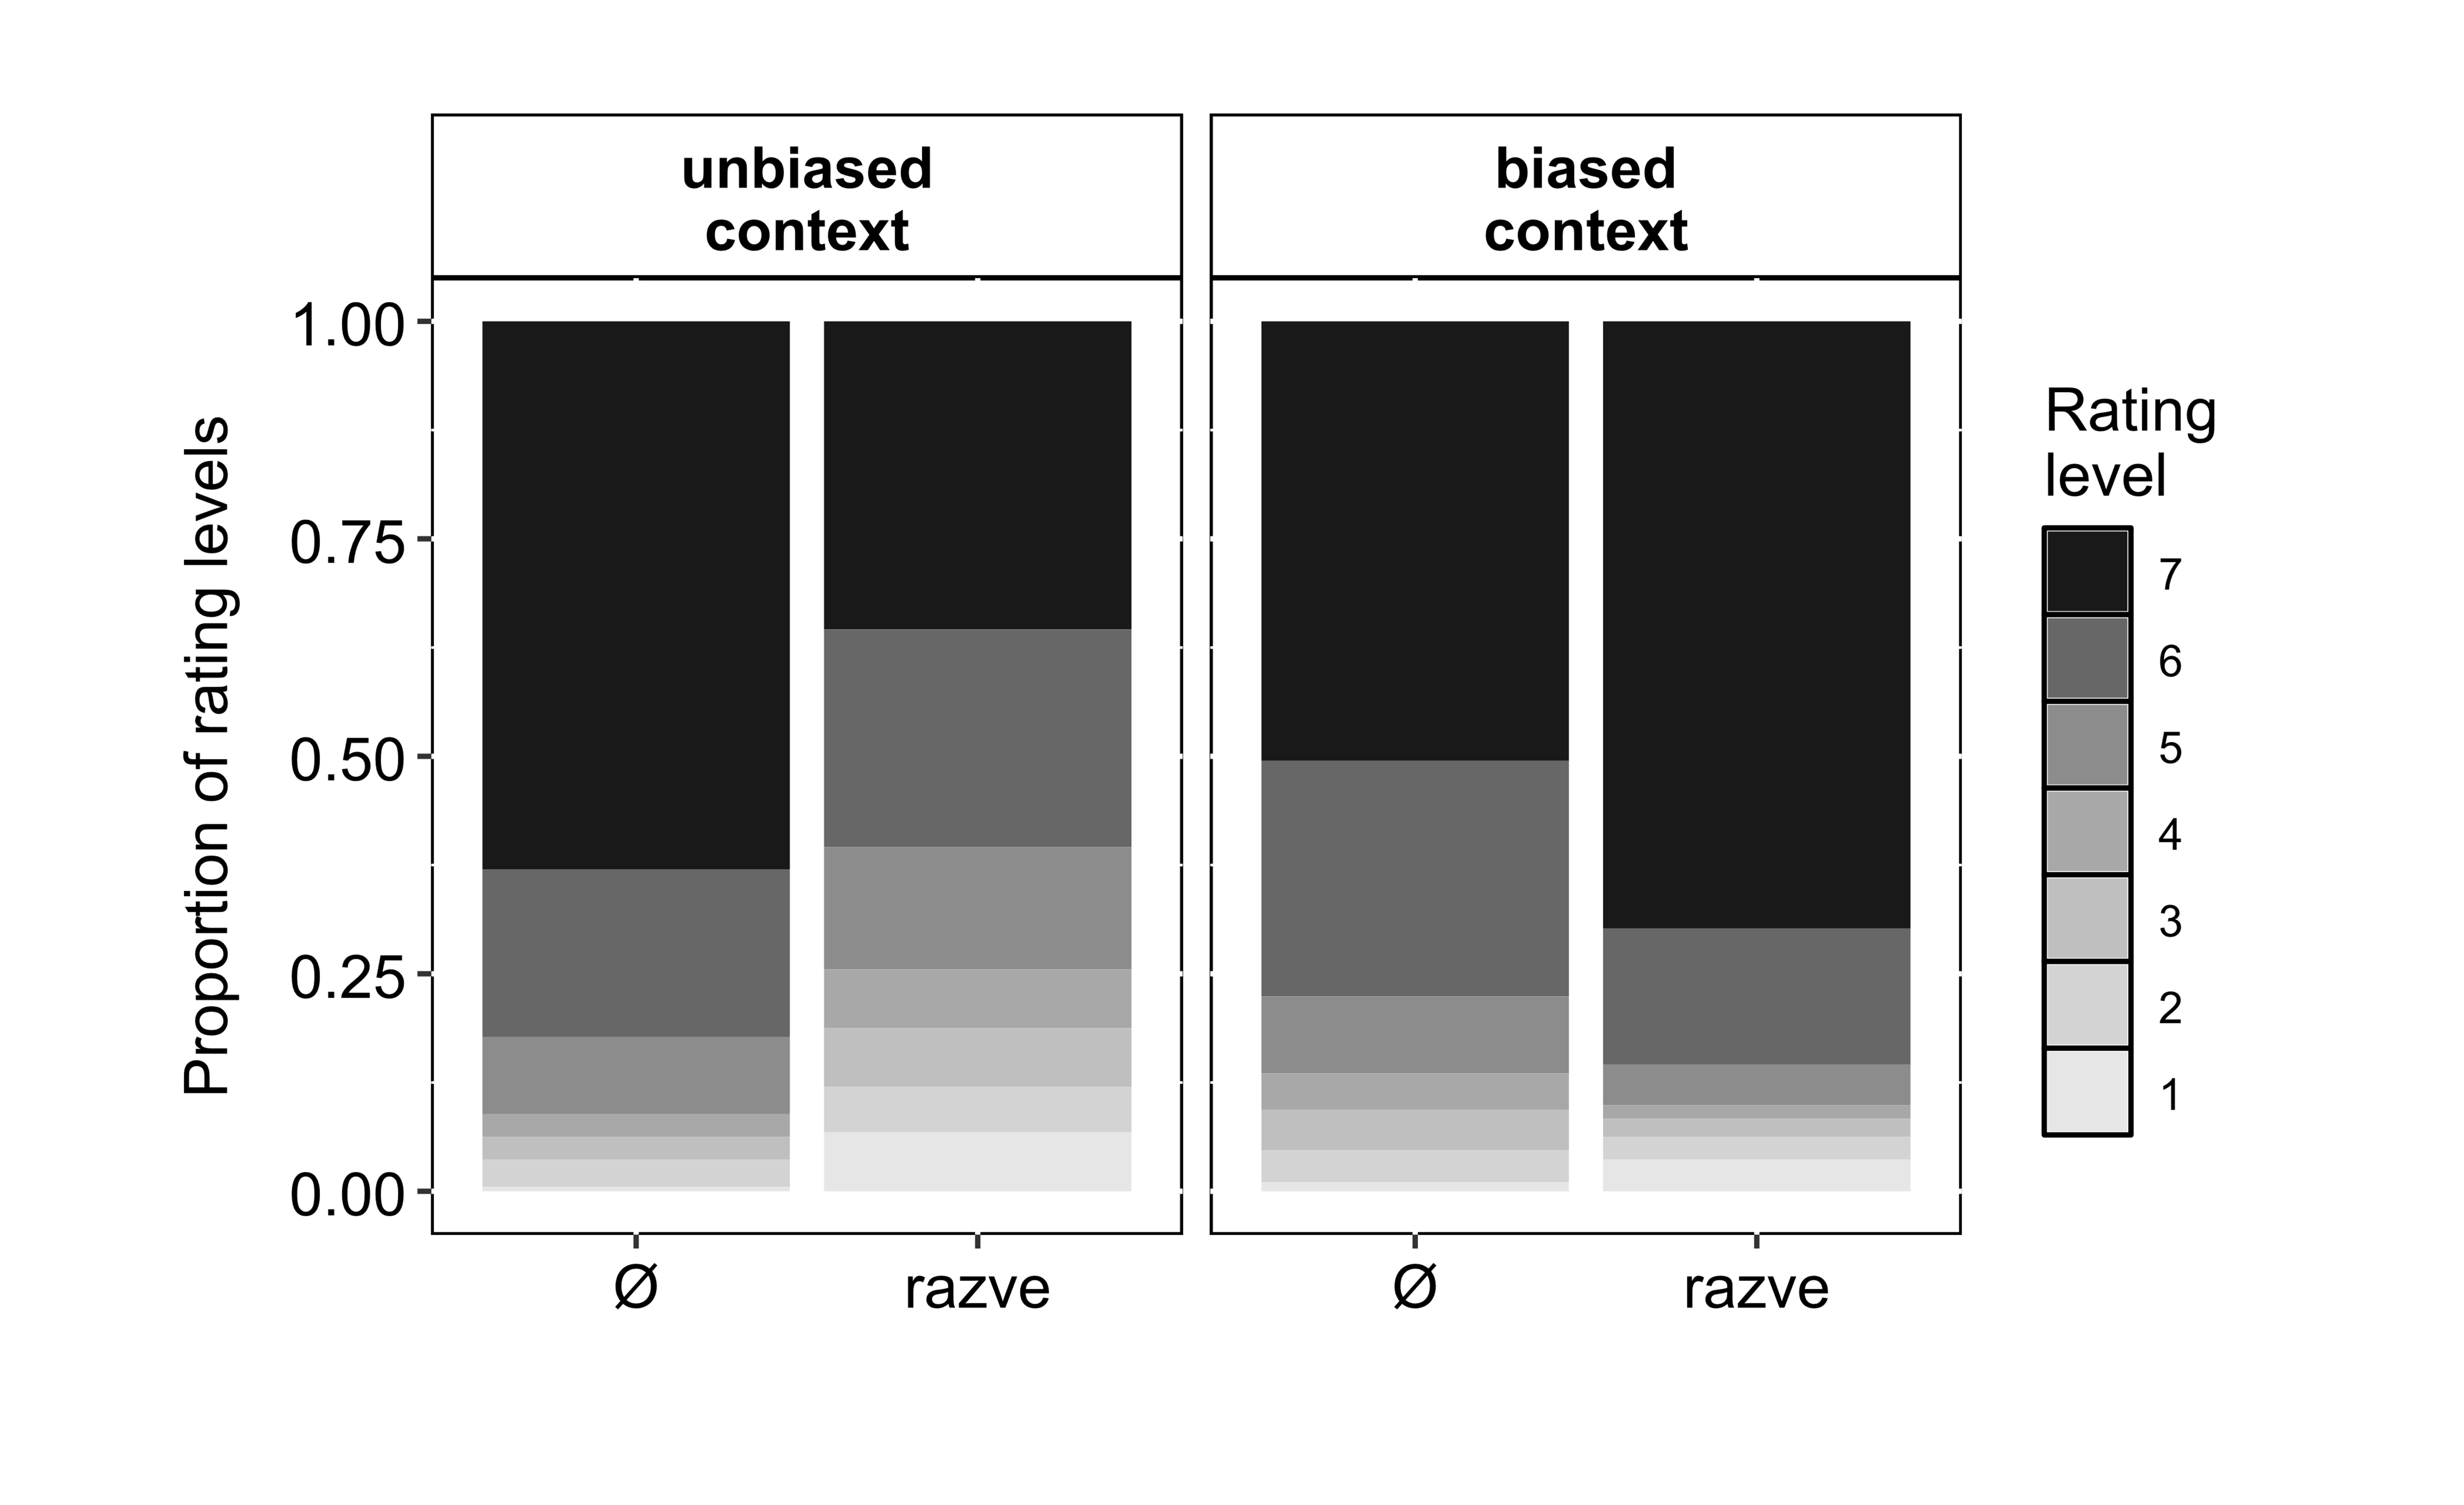
\includegraphics[height=.3\textheight]{figures/ch11-1.png}
\caption{Proportion of rating levels for the experimental conditions in Experiment 1. Darker bars reflect greater contextual appropriateness.}\label{fig:1}
\end{figure}

\tabref{tab:05:6} shows the model estimates for the effect of the two experimental factors. There was a main effect of \textsc{bias context}, which was modulated by an interaction of \textsc{bias context} and \textsc{particle}. We resolved the interaction by forming a subset for \textit{razve}-questions and a subset for bare questions. \textit{Razve}-questions were judged to be more suitable in biased contexts than in unbiased contexts ($\textit{b} = 1.01, \textit{SE} = 0.24, \textit{z} = 4.16,$ $p < 0.001$), and bare questions were judged to be more suitable in unbiased than in biased contexts (\textit{b} = -0.38, \textit{SE} = 0.14, \textit{z} = -2.71, $p$ = 0.0017).\footnote[7]{Due to convergence issues this model did not contain random slopes for lexicalization.}

\begin{table}
\begin{tabularx}{\textwidth}{lYYYl}
\lsptoprule
& estimate & \textit{SE} & \textit{z}-value & \textit{p}-value \\
\midrule
\textsc{bias context} & \phantom{-}0.32 & 0.14 & \phantom{-}2.36 & \phantom{<}0.02* \\
\textsc{particle} & -0.08 & 0.13 & -0.60 & \phantom{<}0.55 \\
\textsc{bias context} $\times$ \textsc{particle} & \phantom{-}0.72 & 0.16 & \phantom{-}4.46 & <0.001*** \\
\lspbottomrule
\end{tabularx}
\caption{Model estimates for the experimental factors in Experiment 1.} \label{tab:05:6}
\end{table}

We checked a potential influence of the actual state of affairs, which was balanced across lexicalizations, because knowing what was actually the case might have influenced participants' judgements: Participants might have developed their own bias(es). The analysis revealed that the questions were judged as less suitable when the action at issue had been carried out, which suggests that the knowledge about the actual state of affairs did influence the assessment of the contextual evidence by the participants. Importantly, there was no interaction with the experimental factors. 

The results for the fillers are given in \figref{fig:2}. We can see that, as predicted for the \textsc{opp.}\textit{razve-uže}\textsc{.neg} fillers, negative \textit{razve}-question with the PPI \textit{uše} are not acceptable in a context with the ``opposite'' bias from the experimental bias contexts, i.e. epistemic bias for $\neg p$ and evidential bias for $p$. The median for these questions is 2, which we take to reflect contextual inappropriateness. \textit{Razve}-questions with \textit{uše} but without negation (\textsc{opp.}\textit{razve-uže}\textsc{.pos}) are suitable in such contexts (median: 7). We take these results to confirm our (uncontroversial) core assumptions regarding the bias profile of \textit{razve}-questions. As the presence of \textit{uže} rather than \textit{eščë} should not play a role for the acceptability of these questions – recall that our corpus investigations showed that both \textit{uže} and \textit{eščë} are felicitous in \textit{razve}-questions –, we assume that it is indeed the altered context that is responsible for these results. Questions with the particle \textit{li} seem to be somewhat degraded in unbiased contexts, although the median is also 7. 

\begin{figure}
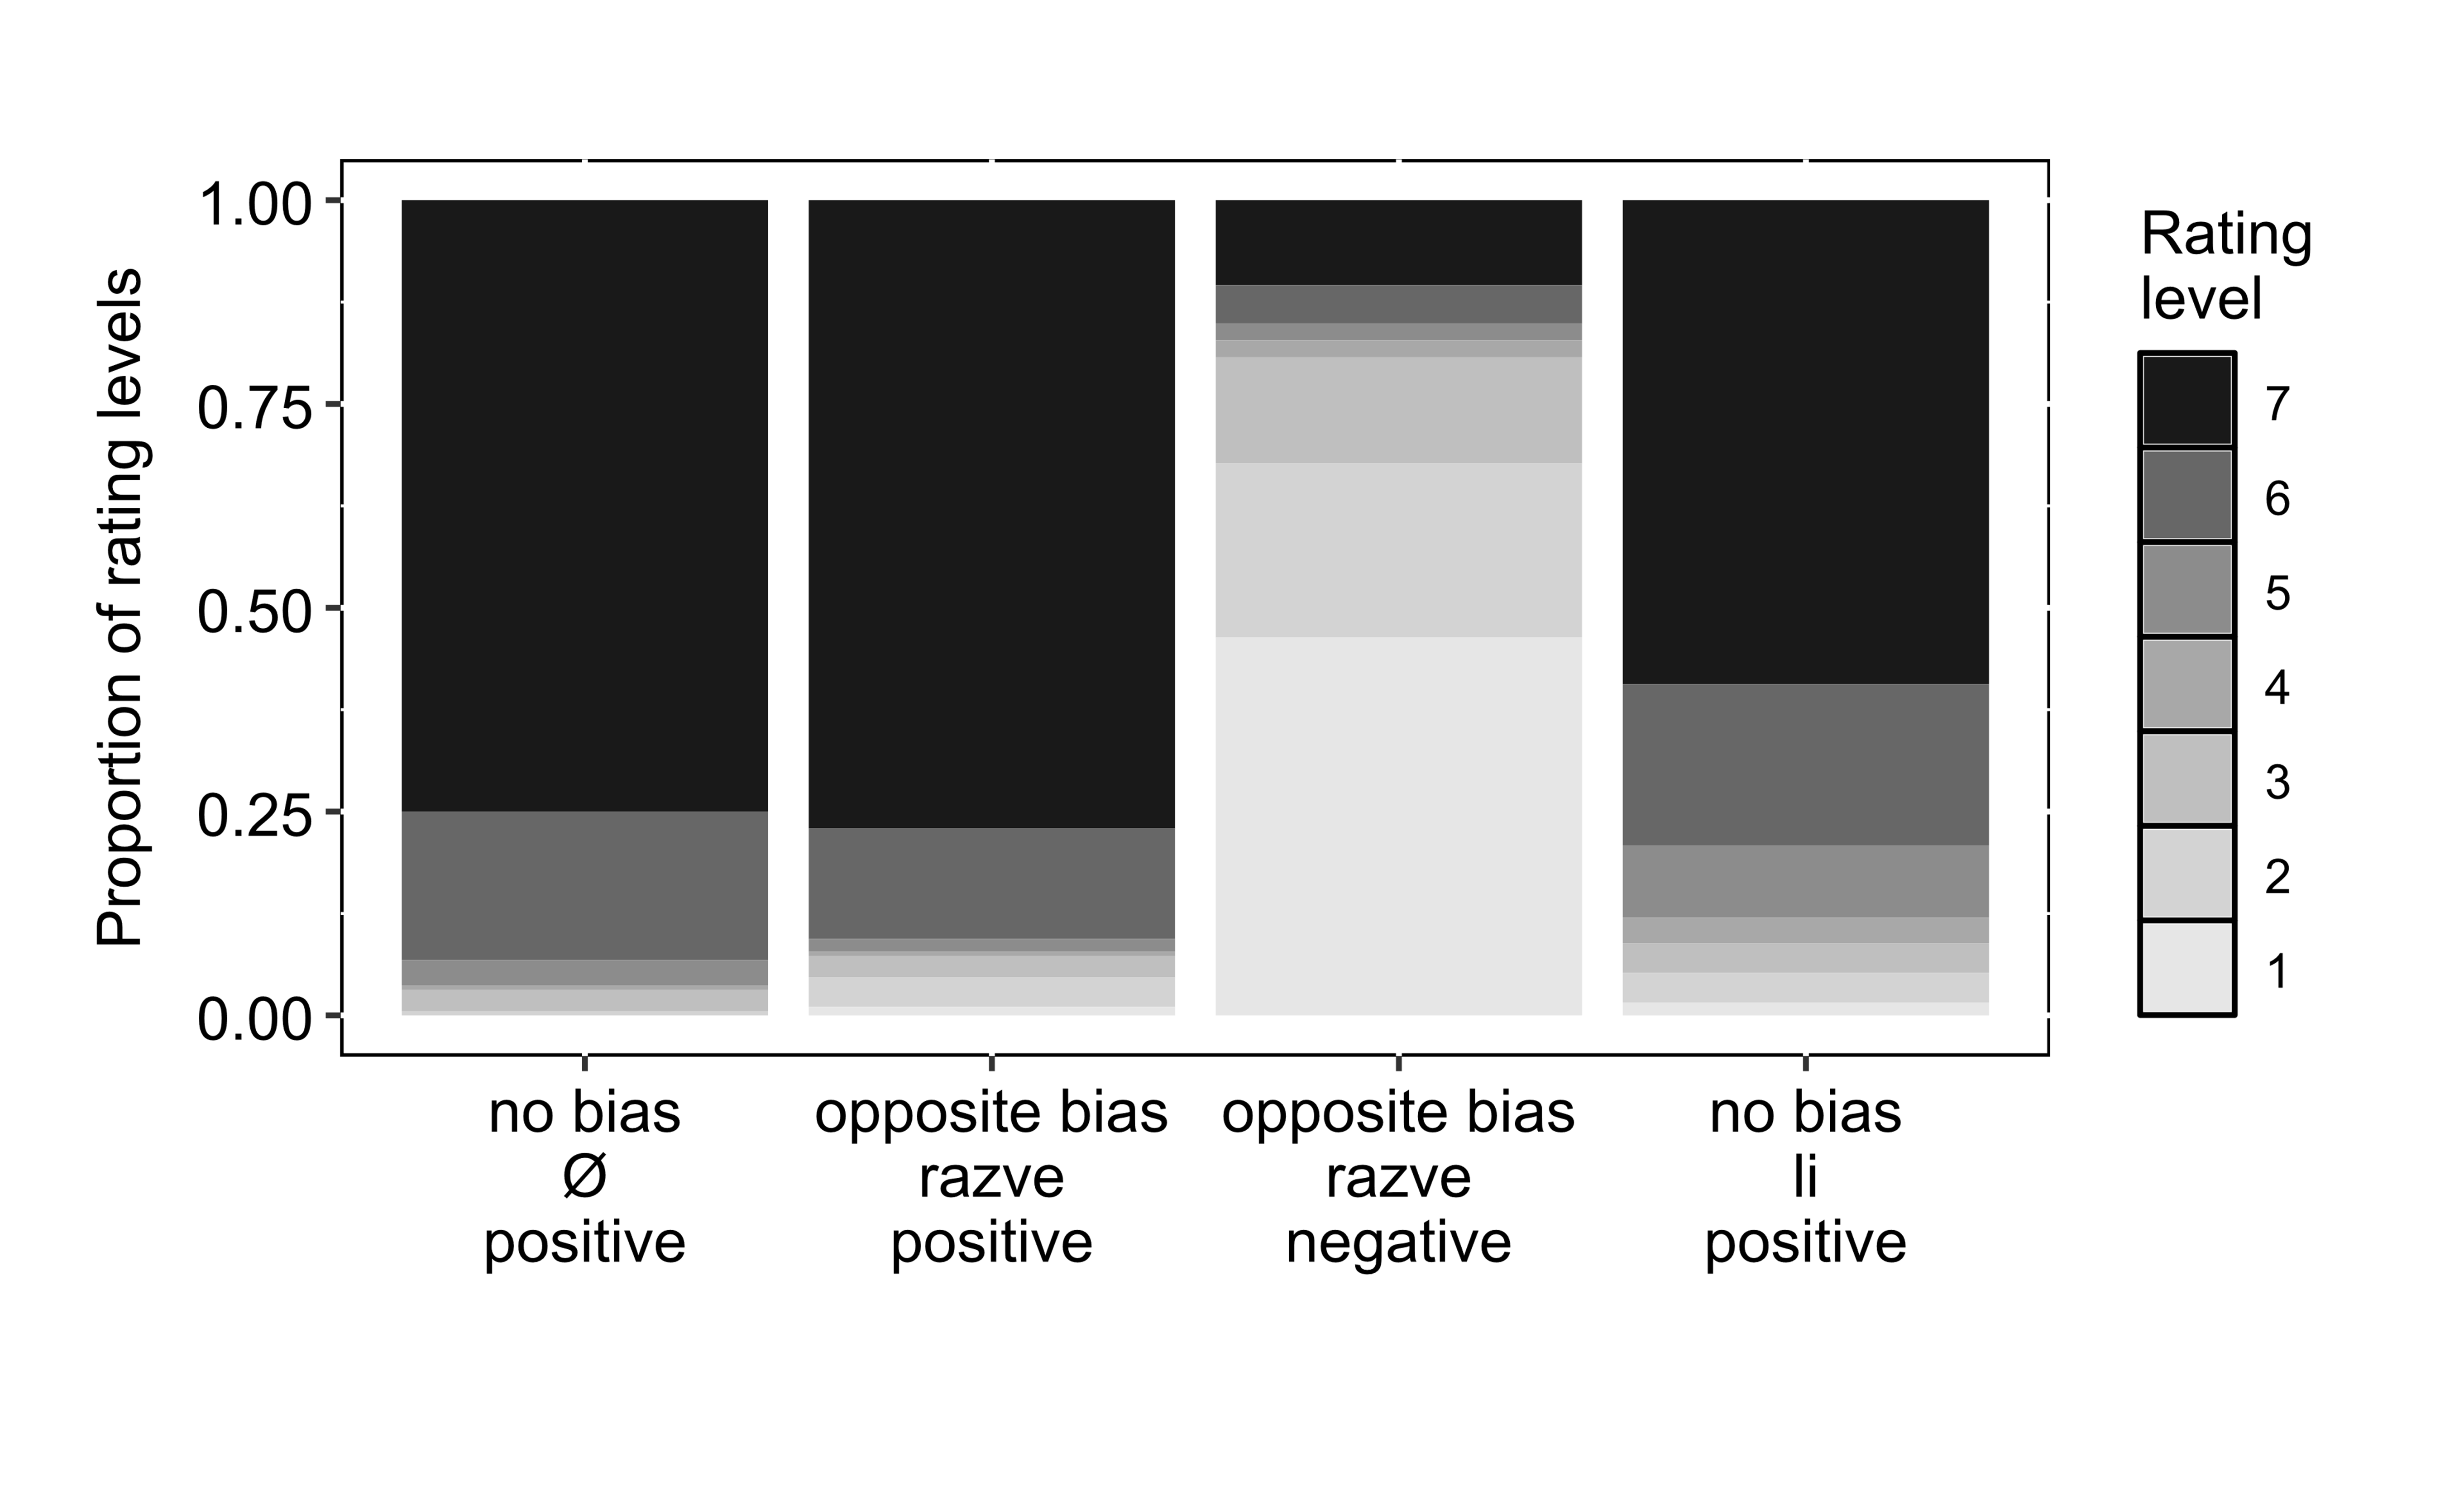
\includegraphics[height=.3\textheight]{figures/ch11-2.png}
\caption{Proportion of rating levels for the four filler types in Experiment 1.}\label{fig:2}
\end{figure}


\subsection{Discussion}\label{sec:05:4:3}

The results suggest that negative polar questions with the weak NPI \textit{eščë} but without a question particle are more acceptable in unbiased list contexts than in contexts with an epistemic bias for $p$ and an evidential bias for $\neg p$ . Negative polar questions with \textit{eščë} and with the particle \textit{razve} are more acceptable in the biased contexts than in the unbiased contexts. The results also indicate that the difference between the question forms in the different context types are small. The median judgement for bare questions in biased contexts is the highest one possible. Similarly, the presence of \textit{razve} in an unbiased list context does not lead to straight contextual inappropriateness: The median judgement is the second-highest possible.

Overall, we interpret the findings from Experiment 1 as supporting our hypothesis that Russian negative \textit{yes-no}-questions without a particle or with the particle \textit{razve} have the contextual appropriateness conditions that we suggested. \textit{Razve}-questions are felicitous in contexts where there is evidence for the prejacent of the question and additionally an epistemic bias for the complement of the prejacent of the question. The question concern is to resolve the conflict between the biases by checking one of them – in questions with \textit{eščë}, this is the evidential bias. Bare questions are most felicitous in contexts where there are no biases for $p$ or $\neg p$. Thus, their contextual appropriateness conditions are more similar to English interrogative questions with non-preposed negation than to English interrogative questions with preposed negation or negative declaratives. Thus, \textit{razve} changes the bias profile of a negative question, as we had hypothesized, but it seems to do that only to a degree. 

Regarding the high acceptability of bare questions in biased contexts, our results suggest that a negative question \textit{per se} – independently of the presence of \textit{razve} – is indeed a more complex and thus a more marked form than a positive question, and a marked form is likely to be interpreted as signalling a marked meaning, for instance a particular bias. Our results suggest that the additional presence of \textit{razve} is not strictly necessary to mark a bias, although it is preferred. Furthermore, our results clearly suggest that the correlation of bias signalling and preposing is language-specific: In Russian there is no preposing. Note, however, that even English or German negative questions presented out of context can be understood as being biased independently of the position of the negation (cf. \citealt{romerohan2004negative}). Future research, especially corpus investigations must show in what contexts bare negative questions in Russian are predominantly used and in how far these contexts come with biases.

Regarding the results for the acceptability of bare questions in unbiased list contexts, we found that they are highly felicitous, as expected. Interestingly, though, they are not actually judged to be ``perfectly'' acceptable in the unbiased contexts: only 82 percent received the highest or the second highest scale point (7: 63\%; 6: 19\%). This contrasts with the bare positive questions in the fillers, 93\% percent of which received the highest scale points (7: 75\%; 6: 18\%). One reason for this finding might be that, as mentioned above, making lists of actions that have not been carried out is, arguably, an unusual activity. A straightforward alternative to making such a list is making a to-do list. It may also be the case, of course, that our experimental manipulation did not make the negative list idea sufficiently prominent for the participants, so that there was room for a biased interpretation of the context. This latter aspect might also be responsible for the fairly high contextual acceptability of \textit{razve}-questions in the unbiased contexts. Another aspect that might contribute to explaining this finding is that participants may always interpret \textit{razve}-questions as biased and assume that the speaker will have had a reason to express the bias – due to previous beliefs that are not mentioned in the scene-setting passage but that might be present in the larger conversation. Participants might thus just enrich the context as they see fit. 

\section{Experiment 2: \textit{Razve} vs. \textit{neuželi}}\label{sec:05:5}

In Experiment 2, we explored the idea that questions with the particles \textit{razve} and \textit{neuželi} have the same bias profile but signal different concerns of the question, as discussed in \sectref{sec:05:3}. Specifically, we investigated the source and presumed strength of the biases, which by hypothesis impact the extent of the conflict between the biases as experienced by the speaker, and his/her psychological state (emotional attitude). In Experiment 1, the source for the epistemic bias for $p$ in \textit{razve}-questions was left unspecific: Katja in \xref{16} just thought that something was the case, and in other experimental items assumptions, beliefs etc. were mentioned. The source for the evidential bias was an utterance by Dima, which suggested that there might be evidence for $\neg p$. Thus both biases had rather weak sources and were based on indirect signs rather than direct observation. There was no indication of a major conflict experienced by the person asking the question, Katja. In Experiment 2, we manipulated the above-mentioned ingredients of question concern for \textit{razve} vs. \textit{neuželi}-questions.

On the basis of our considerations in \sectref{sec:05:3}, we hypothesized that \textit{razve}-questions are \textit{checking questions}, and that \textit{neuželi}-questions are \textit{disbelieving questions} (also see \sectref{sec:05:3:3}). \tabref{tab:05:7} summarizes how we implemented these hypotheses by manipulating various parameters in the scene-setting passage. 

\begin{table}
\begin{tabularx}{\textwidth}{L{4.25cm}L{3.5cm}L{3.5cm}}
\lsptoprule
& \phantom{checki}\textit{razve} & \phantom{disbelie}\textit{neuželi} \\
& checking question & disbelieving question \\
\midrule 
conflict between speaker preference and likely true state of affairs & \phantom{checki}weak & \phantom{disbelie}strong \\
\midrule 
epistemic bias for $p$ & based on one piece of direct evidence in one previous situation & based on a general belief that builds on experience gathered in many previous situations \\
\midrule 
evidential bias for $\neg p$ & based on one piece of indirect but plausible evidence & based on one piece of fairly unequivocal evidence\\
\midrule
psychological state & doubt, uncertainty & irritation, puzzlement,\\
(speaker attitude) & & disbelief\\
\lspbottomrule
\end{tabularx}
\caption{Meaning contributions of \textit{razve} and \textit{neuželi} in terms of bias source, speaker attitude, and ensuing conflict between speaker preference and likely true state of affairs as assessed by the speaker.}\label{tab:05:7}
\end{table}

For \textit{razve}-questions, i.e. checking questions, we assumed that the (psychological) conflict experienced by the speaker is weak (similar to Experiment 1). The source of the epistemic bias is the speaker's previous observation of a single piece of direct evidence for $p$. The evidential bias for $\neg p$ is indirect but potentially plausible. Due to this constellation, the speaker has doubts s/he wishes to dispel. For \textit{neuželi}-questions, i.e. disbelieving questions, we assumed that the (psychological) conflict the speaker experiences is strong. The epistemic bias for $p$ stems from a rather firmly held belief that has developed from multiple previous observations, i.e. from general experience in the past. Recall from \sectref{sec:05:3} that we do not follow  \quotecite{baranov86} suggestion that assumptions which are not based on direct observation can only provide weak support for epistemic bias. Rather, we think that firm beliefs can be built on the basis of common experience and reasoning about what the world is like in general. This will then have consequences for the speaker's beliefs about individual situations. The source of the evidential bias for \textit{neuželi}-questions is unequivocal, more or less direct evidence in the contextual situation. The speaker is puzzled or irritated because s/he has a preference for keeping the original belief which in view of the evidence seems difficult.

\subsection{Method}\label{sec:05:5:1}
Like in Experiment 1, participants in Experiment 2 read short scenarios, consisting of a scene-setting passage leading up to a conversation starting with a question. Experiment 2 had a $2\times2$ design with the factors \textsc{bias context} (or question type): \textit{checking question context} vs. \textit{disbelieving question context}, and \textsc{particle} (\textit{razve} vs. \textit{neuželi}). An example is given in \xref{ex:05:14}.

\begin{exe}
\ex \label{ex:05:14} In the village where Dima and Katja live, there is a very old oak tree that is to be cut down. Dima and Katja have organised a citizen's committee and are opposing the cutting down of the tree. Julja, their friend and an environmental activist, helps them prepare leaflets. This afternoon, Dima spoke to Julja and found out that she has already written the text for the leaflets. After lunch, Dima is talking with Katja.
\sn \textit{Checking question context:} Katja saw Julja put some text on Petja's desk. She thought it was a ready-made text for the leaflets, but now she has doubts as Dima has just told her that he wanted to offer Julja help. To dispel her doubts, Katja asks:
\sn \textit{Disbelieving question context:} Julja is usually very quick with her tasks, so Katja was sure that the text for the leaflets was ready a long time ago, and today she agreed with her friends to hang them up. But when she heard from Dima that he wanted to offer Julja help with preparing the leaflets, she was puzzled and asked:
\sn Katja: \gll {Razve / Neuželi} Julja eščë ne napisala tekst dlja listovok?\\
\textsc{part} Julja yet not wrote text for leaflets\\
\glt \phantom{Katja:} `Has Julja really not written the text for the leaflets yet?'
\end{exe}

The experiment contained 24 lexicalizations in four conditions. As in Experiment 1, the actual state of affairs was balanced across the lexicalizations, and there were 24 filler lexicalizations in four types, all of which contained the PPI \textit{uže} `already'. Three of the filler types were the same as in Experiment 1: \textsc{opp.}\textit{razve-uže}\textsc{.neg}, \textsc{opp.}\textit{razve-uže}\textsc{.pos} and \textsc{nobias.}\textit{uže}\textsc{.pos}. The fourth type, containing \textit{n\-eu\-že\-li}, had the same bias context as the experimental conditions but \textit{neuželi} occurred in a negative question with \textit{uže} (\textit{neuželi-uže}\textsc{.neg}). The filler types \textsc{opp.}\textit{raz\-ve}\textit{-uže}\textsc{.neg} and \textit{neuželi-uže}\textsc{.neg} were expected to be unacceptable: the first one because the bias is inappropriate (replication of Experiment 1), the second one because according to our deliberations in \sectref{sec:05:3:2} \textit{neuželi} seems to be incompatible with \textit{uže} in negative questions unless \textit{uže} scopes over the negation, which was not a plausible reading in these filler items.

The 48 lexicalizations were distributed over four lists in a Latin square design so that each list contained 24 experimental and 24 filler items. In addition, there were two practice items on each list. 

The task of the participants was the same as in Experiment 1. Experiment 2 was also run as a web experiment on \textit{soscisurvey.de}. 35 participants (26 female, 9 male; mean age: 34.7; age range: 18--56) with Russian as their native language were recruited via \textit{prolific.com}. Before taking part in the experiment, participants gave informed consent. They were paid for participation.

\subsection{Results}\label{sec:05:5:2}

The data from three participants were excluded from the statistical analysis based on our exclusion criteria. This left the data from 32 participants for analysis. Four individual experimental items had to be excluded because there was a text error, which was detected and reported to us by one participant early on and subsequently corrected. This left 764 experimental items for the analysis.

\begin{figure} 
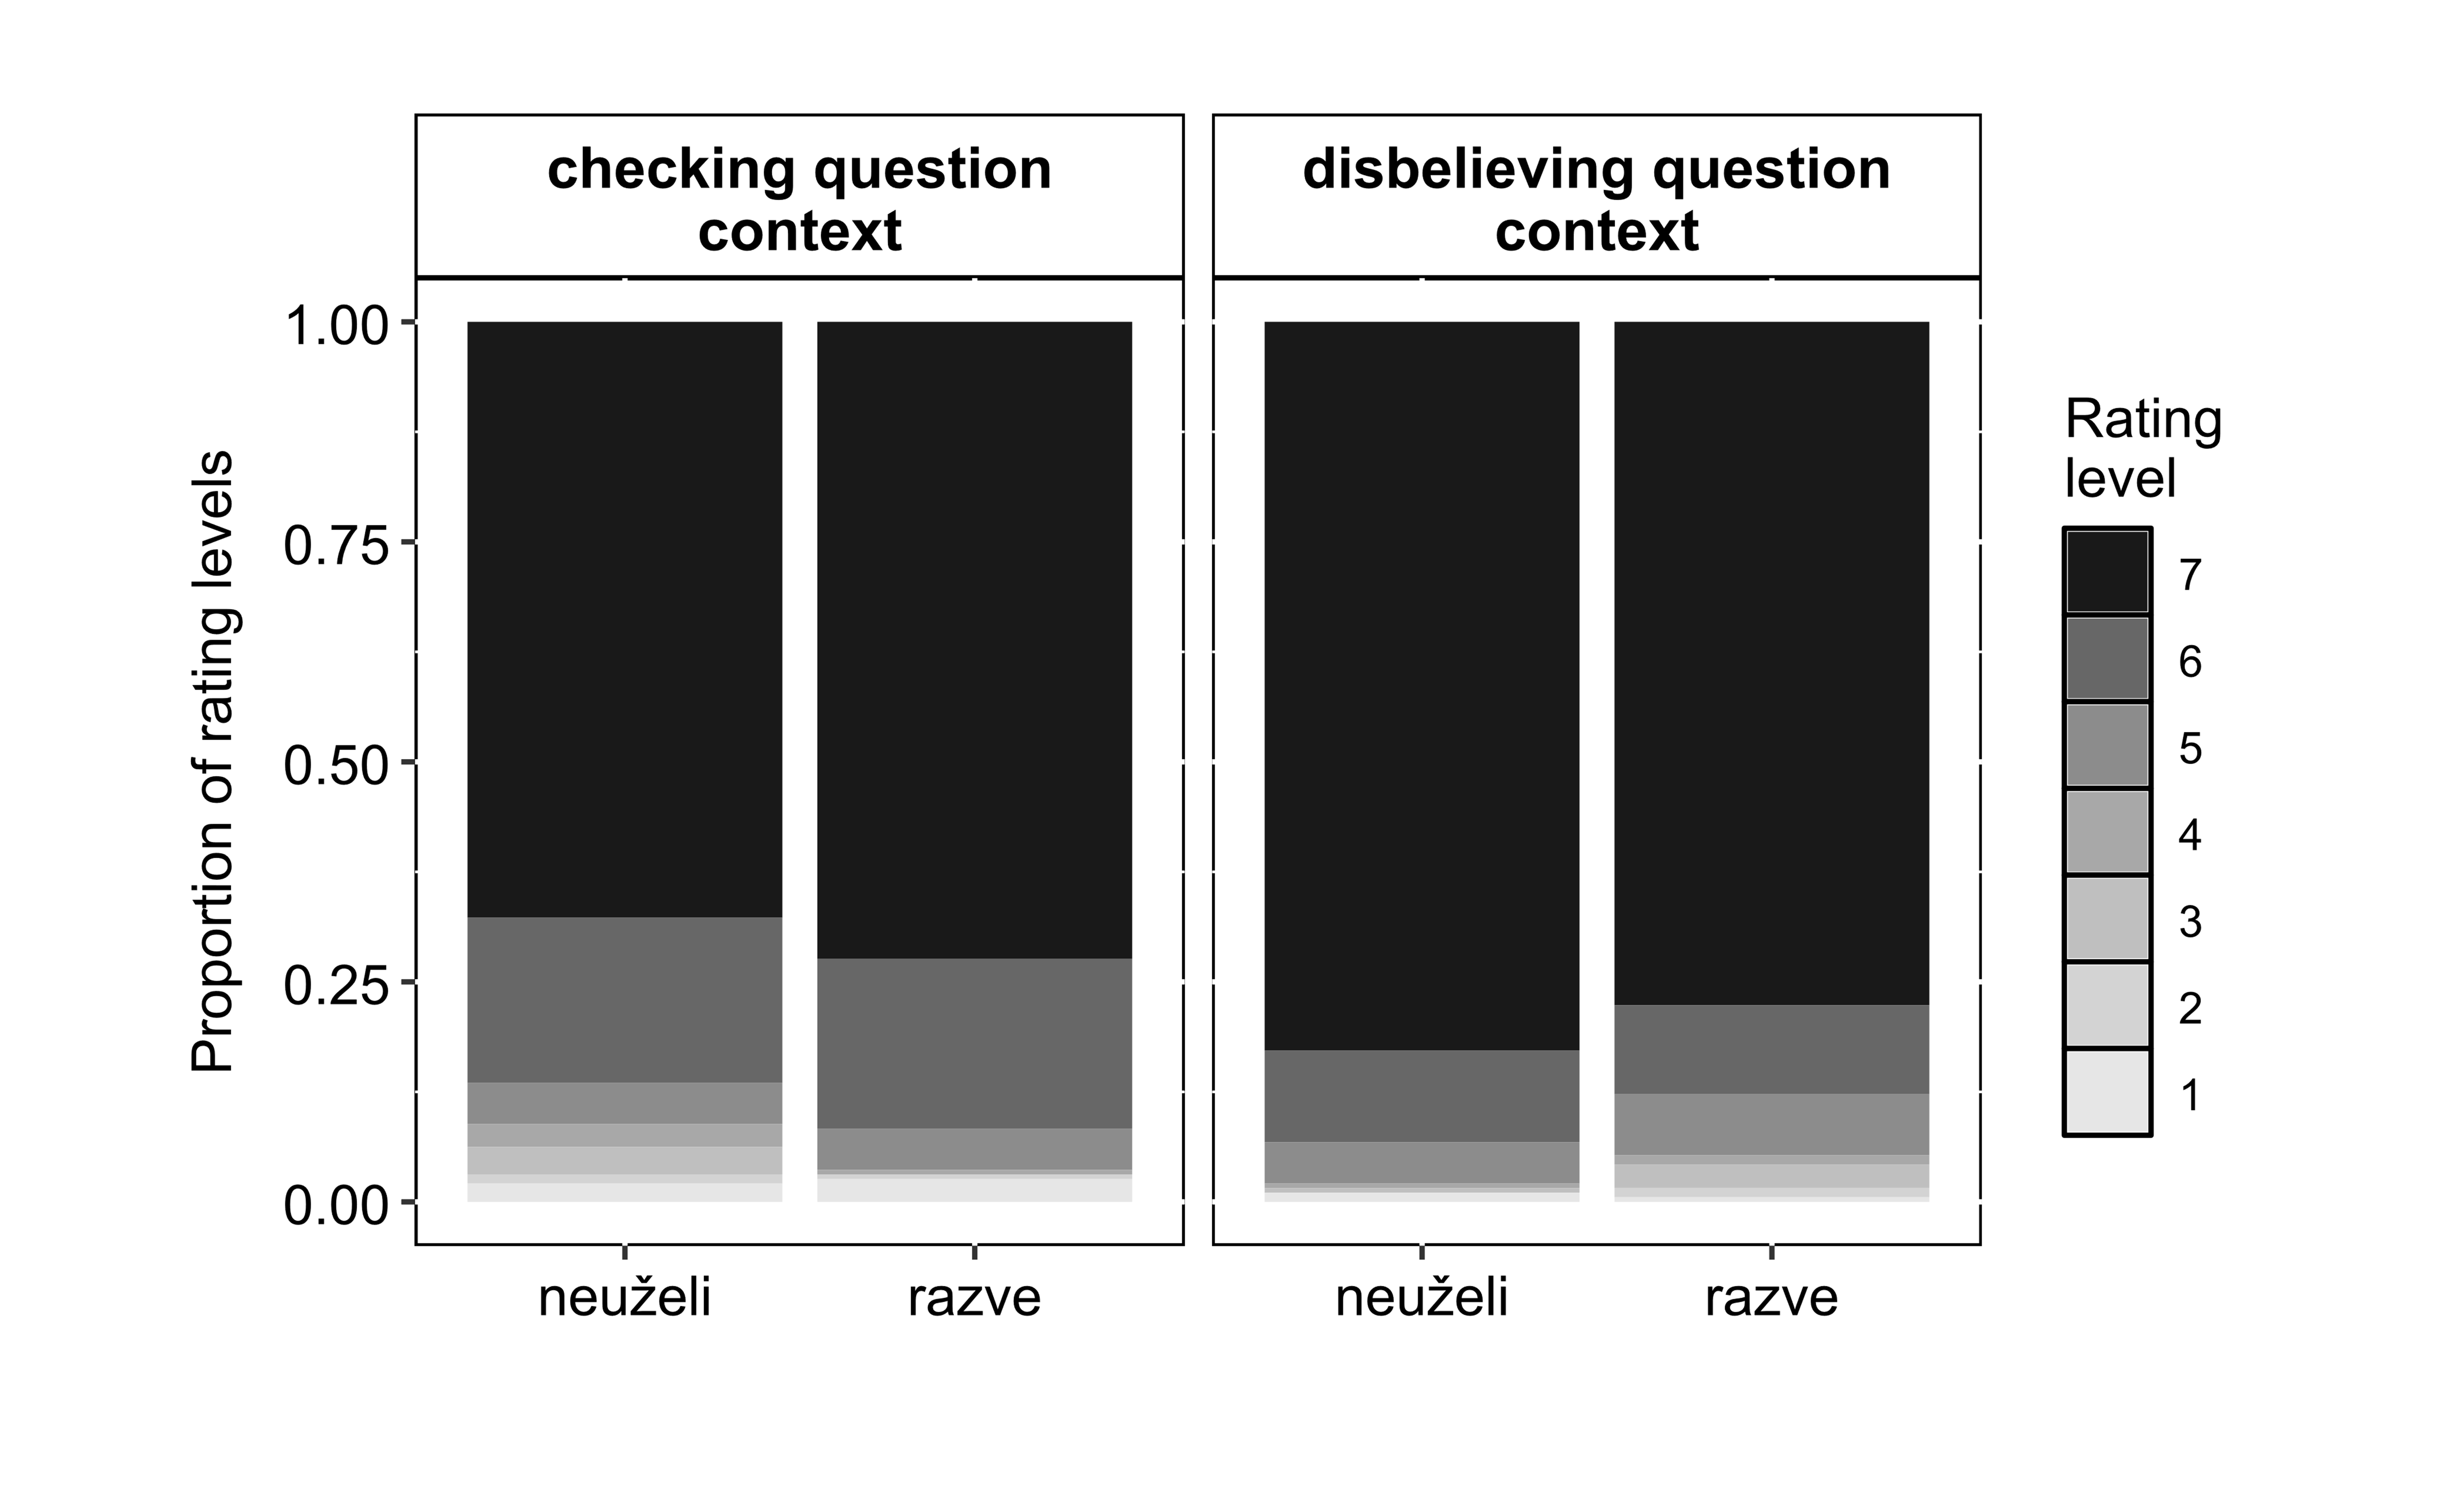
\includegraphics[height=.3\textheight]{figures/ch11-3.png}
\caption{Proportion of rating levels for the experimental conditions in Experiment 2.} \label{fig:3}
\end{figure}

As in Experiment 1, the statistical analysis was conducted by fitting a cumulative link mixed model for ordinal data (R package ordinal, \citealt{christ19}). \textsc{bias context} and \textsc{particle} were fixed factors. They were sum-coded. Participant and lexicalization were random factors. The final, maximal model contained random intercepts and slopes for the experimental factors and their interaction.  

\figref{fig:3} shows the results for the experimental conditions in terms of proportions of rating levels. The median for all target questions was 7. \tabref{tab:05:8} shows the model estimates for the effects of the two experimental factors. There was a main effect of \textsc{bias context}, and a marginal interaction of \textsc{bias context} and \textsc{particle}. Overall, the questions were judged to be more suitable in the disbelieving question contexts. To explore the effect of \textsc{bias context} for the two particles separately, we resolved the interaction by subsetting the data by \textsc{particle}. The analysis revealed that the effect was only significant for the questions with \textit{neuželi} (\textit{b} = 0.65, \textit{SE} = 0.15, \textit{z} = 4.23, $p$ < 0.001 (model with intercepts only)).

\begin{table}
\begin{tabularx}{\textwidth}{lYYYl}
\lsptoprule
& estimate & \textit{SE} & \textit{z}-value & \textit{p}-value \\
\midrule
\textsc{bias context} & \phantom{-}0.50 & 0.20 & \phantom{-}2.58 & <0.01** \\
\textsc{particle} & -0.24 & 0.21 & -1.13 & \phantom{<}0.260 \\
\textsc{bias context} $\times$ \textsc{particle} & -0.35 & 0.19 & -1.84 & \phantom{<}0.066 \\
\lspbottomrule
\end{tabularx}
\caption{Model estimates for the experimental factors in Experiment 2.} \label{tab:05:8}
\end{table}

As in Experiment 1, we explored the influence of (the balancing factor of) the state of affairs on the judgements of the participants. The questions were judged as slightly less suitable when the action at issue had been carried out. There was no interaction with the experimental conditions. 

The results for the fillers are given in \figref{fig:4}. These replicate the findings of Experiment 1 for the three left-most filler types in the figure (medians 7, 7 and 2, from left to right). The new filler type, on the right, received low acceptability ratings, as predicted (median = 2). 

\begin{figure} 
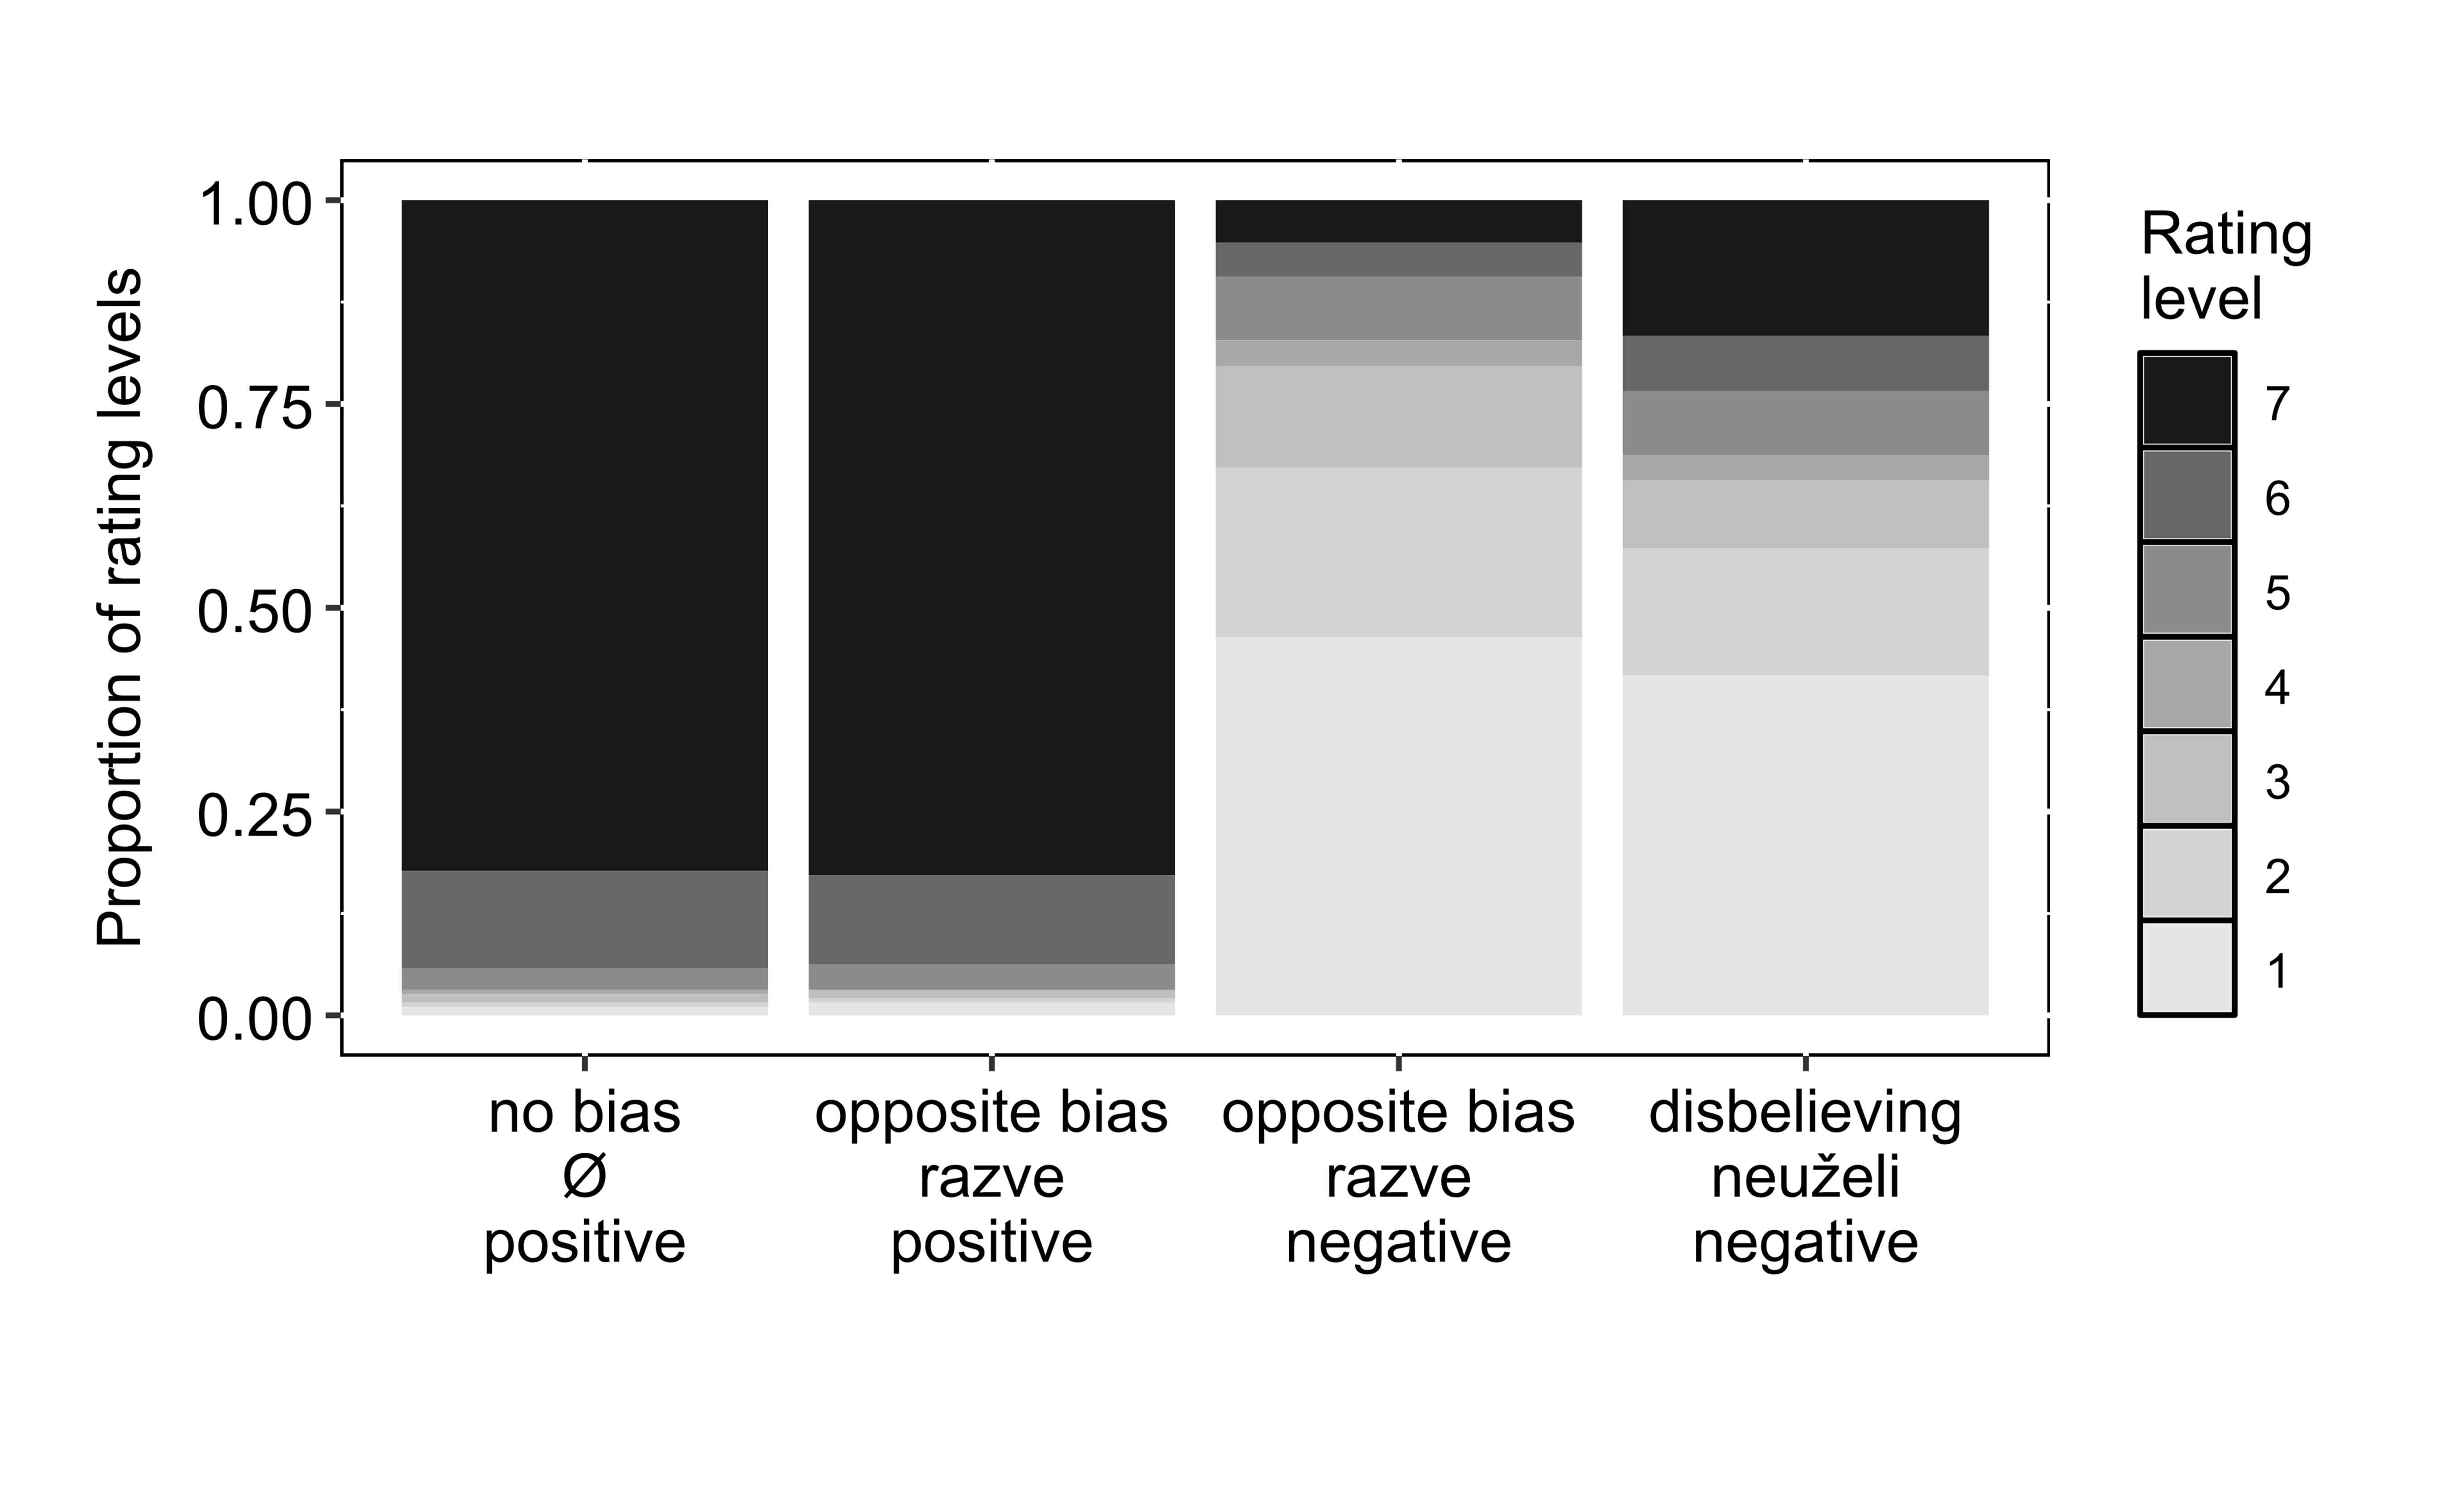
\includegraphics[height=.3\textheight]{figures/ch11-4.png}
\caption{Proportion of rating levels for the filler types in \newline
Experiment 2.} \label{fig:4}
\end{figure}

\subsection{Discussion}\label{sec:05:5:3}

The results of Experiment 2 indicate that our manipulation of the context with respect to the source and strength of the biases as well as of the psychological state of the speaker produced small effects on the acceptability of the questions under investigation. For \textit{neuželi}-questions we found that they are more acceptable in contexts where the question concern includes expressing disbelief of the contextual evidence than in contexts where the question concern includes double-checking the evidential bias and dispelling doubt that has come up in view of the contextual evidence. This finding supports our hypothesis concerning \textit{neuželi}-questions, but we note that the difference between the context types is small. It is clearly not the case that \textit{neuželi}-questions are unacceptable in checking question contexts. As a matter of fact, 86.5 percent of the \textit{neuželi}-questions received a median corresponding to one of the two highest scale points (7: 67.7\%; 6: 18.6\%) in these contexts, in comparison to 93 percent in disbelieving question contexts (median of 7: 82.8\%; 6: 10.4\%). We take this to mean that \textit{neuželi}-questions are acceptable in both contexts with a slight preference for our rendering of disbelieving question contexts. For \textit{razve}-questions we found no effect. These questions were highly acceptable in both contexts: 92 percent of the \textit{razve}-questions received a very high median in the checking-question context (7: 72.4\%; 6: 19.3\%), and 88 percent in the disbelieving question context (7: 77.7\%; 6: 10.1\%). It is clear that the judgements for \textit{razve}-questions in our rendering of disbelieving question contexts are far away from any kind of contextual inappropriateness.

Overall, our results suggest that the manipulation of the question concern that we applied makes some difference but only a small one. There might be several reasons for this. It is possible that the conflict between the speaker's original belief and the apparent state of affairs in the disbelieving question context was not strong enough to make \textit{razve} inappropriate. Similarly, the doubt described in the checking question context still allowed an accommodation of an irritated or indignant psychological state of the speaker. We assume that the participants in the experiment, being cooperative language users, applied an accommodation strategy and enriched the context situation in order for the respective particle to match the context. This assumption needs to be tested in future research with different research methodologies, such as a forced choice experiment (choice: \textit{razve} vs. \textit{neuželi}) mimicking production. Importantly, our conceptual deviation from \quotecite{baranov86} claim that reasoning does not create strong beliefs cannot be responsible for the results because we still applied the difference between direct observation vs. reasoning that Baranov identified as crucial for the choice between \textit{razve} vs. \textit{neuželi} in the creation of the experimental conditions.

Briefly turning to our proposal regarding the restriction of \textit{neuželi}-questions to inner negation readings (\sectref{sec:05:3:2}), recall that we double-checked this in the fillers with \textit{neuželi}-questions containing \textit{uže} in our usual biased context. As expected, these questions were judged to be unacceptable. We suggest that the reason is indeed the presence of \textit{uže} because – as we just saw – the same type of question with eščë is highly acceptable. This finding supports our proposal that \textit{neuželi}-questions cannot contain outer negation – which would be compatible with the PPI \textit{uže}. \textit{Neuželi}-questions can only contain inner negation: They express disbelief in the truth of a negative proposition, the evidence that $\neg p$.

\section{General discussion}\label{sec:05:6}

Overall, our investigation has shown that negative questions without a particle, with the particle \textit{razve} and with the particle \textit{neuželi} are all felicitous in contexts supporting an evidential bias for the proposition denoted by the prejacent of the question, $\neg p$, and an epistemic bias for the complement of that proposition, $p$. However, they differ in the degree of felicity. 

Bare negative questions are most acceptable in contexts without such a bias, that is in negative list contexts. The particle \textit{neuželi} seems to be most acceptable if the conflict between epistemic and evidential bias experienced by the speaker is strong rather than weak, and if the speaker does not want to accept what the evidence suggests. So \textit{neuželi} is particularly well-suited to mark a disbelieving question, and it is better suited to mark a disbelieving than a checking question. Furthermore, on the basis of our qualitative corpus investigation, on the basis of the Russian versions of \textit{too/either-}questions \xxref{ex:05:13}{16}, and on the basis of the experimental results for the fillers, we argued that \textit{neuželi} cannot occur in questions with outer negation, even in a context supporting the bias and question concern that by hypothesis are appropriate for an outer negation reading. In sum, we thus suggest that the concern of a \textit{neuželi}-question is about the evidence in the situation: this is what is ``disbelieved''. The concern of the question is to find out whether the evidence can be believed, because it is unexpected and because of the speaker's desire to keep his/her original belief (epistemic bias). For \textit{razve} we did not find differences in the felicity between disbelieving and checking questions. The concern of a \textit{razve}-question is just to dispel doubt. To achieve that, it can either double-check the evidential bias (inner negation reading) or the epistemic bias (outer negation reading).

In view of the small differences in our experimental results, it is important to highlight that \textit{double-checking} evidence and \textit{signaling disbelief} in evidence eventually are very similar question concerns. Thus, in the end it is not surprising that \textit{razve} vs. \textit{neuželi}-questions are similarly appropriate in the same contexts. We mentioned this issue in several places before: readers may accommodate subtle shades of meaning. Note that this also holds for the fairly high felicity of bare negative questions in biased contexts, which we addressed in our discussion of Experiment 1. The mere presence of a negation might trigger an interpretation of a question as signaling some bias, which readers may do by accommodating richer contexts. This issue is an interesting methodological challenge for experimental investigations of contextual felicity, which must be addressed in future research.

In the remainder of this section, we will address the difference between \textit{razve} and \textit{neuželi} in their (in)ability to double-check the epistemic bias. This difference is interesting for theories of inner and outer negation. We will put forth a theoretical proposal that accounts for the difference but for space reasons will not discuss other theories on question bias and question concern.\footnote[8]{Checking question and disbelieving questions of sorts have been discussed under the labels \textit{confirmative} and \textit{incredulous} questions (e.g. \citealt{jeong18, rudin18, goodhue21:lsa}).} Our proposal builds on accounts of biased questions which assume that such questions contain conversational epistemic operators \citep{romerohan2004negative, Repp06, repp_negation_2009, Repp13, Romero15}. \citet{romerohan2004negative} suggest that preposed negation obligatorily introduces a conversational epistemic operator \textsc{verum} (based on \citealt{hoehle88, hohle_uber_1992}), which expresses that the speaker is sure that the proposition in its scope should be added to the common ground. A question with \textsc{verum} thus asks whether or not the speaker is sure that a given proposition should be added to the common ground. \textsc{Verum} interacts scopally with the negation operator, see \xref{read:neg}. \textsc{Verum} may scope under negation \xref{read:neg:out}, which produces an outer negation reading: the question asks whether the positive proposition in the scope of \textsc{verum} should not be added to the common ground. \textsc{Verum} may also scope over the negation \xref{read:neg:inner}, which produces an inner negation reading: the question asks whether the negative proposition in the scope of \textsc{verum} should be added to the common ground. Regarding non-preposed negation, Romero \& Han suggest that biased readings are possible – as we mentioned earlier –, thus, we assume that preposing is not required to signal the presence of \textsc{verum}.

\ea \label{read:neg}
\ea \label{read:neg:out}
Outer negation reading 
\sn {[\textsc{q} [\textit{neg} \textsc{verum} [$p$]]]} = $\{\textit{neg} \textsc{ for-sure-add } p, \neg\textit{ neg} \textsc{ for-sure-add } p \}$
\ex \label{read:neg:inner}
Inner negation reading
\sn {[\textsc{q} [\textsc{verum} [\textit{neg} $p$]]]} = $\{\textsc{ for-sure-add } \textit{neg } p, \neg\textsc{ for-sure-add } \textit{neg } p \}$
\z
\z

\citet{Repp06, repp_negation_2009} discusses some difficulties of Romero \& Han's \textsc{verum} account for outer negation readings and suggests that outer negation is better analysed as involving a kind of negative counterpart of \textsc{verum}, namely \textsc{falsum}. \textsc{Falsum} expresses that the speaker is sure that the proposition in its scope should not be added to the common ground (also see \citealt{Romero15}). \textsc{Falsum} is denoted by the negation marker in an outer negation question. It thus scopes over a positive proposition (unless there are several negation markers). For inner negation, Repp keeps Romero \& Han's \textsc{verum} analysis. \textsc{Verum} and \textsc{falsum}, being illocutionary operators, always scope over all propositional operators. \xref{ex:05:op} shows the difference between the two negation readings in Repp's account. Note that the occurrence of PPIs in outer negation questions, and of NPIs in inner negation questions is predicted by both accounts because only in the latter is there propositional negation.

\ea \label{ex:05:op}
\ea \label{ex:05:op:out}
Outer negation reading: [\textsc{q} [\textsc{falsum} [$p$]]]
\ex \label{ex:05:op:in}
Inner negation reading: [\textsc{q} [\textsc{verum} [\textit{neg} $p$]]]
\z
\z

\largerpage
We propose that this account can be applied to Russian. As for English, we assume that it is not necessary to have preposed negation in a question with \textsc{verum} or \textsc{falsum}, which is an option that is not available in Russian anyway due to the syntax of negation in this language. We assume that the mere presence of a negative marker is sufficient to signal the presence of \textsc{verum} or \textsc{falsum}. However, recall from Experiment 1 that even though bare negative questions are fairly felicitous in biased contexts, they are less felicitous than \textit{razve}-questions. This observation can be explained if we assume that when choosing between question forms the speaker will choose the better (or best) option. This better option would be a \textit{razve}-question. To explain why this might be the case, we turn to the meaning contributions of \textit{razve} and \textit{neuželi}.

Recall that both particles can roughly be translated as `really'. \citet{romerohan2004negative} observe that English \textit{really} is only compatible with inner negation. They show this for non-preposed negation and polarity-sensitive additive particles, see \xref{ex:05:neg:out:a} and \xref{ex:05:neg:in:a}. Romero \& Han suggest that \textit{really} is an instantiation of the conversational epistemic operator \textsc{verum}. If we assume with \citet{Repp06, repp_negation_2009, Repp13} that outer negation is \textsc{falsum}, the fixed scope relation \textit{really} > \textit{negation} (inner negation) is predicted because \textsc{falsum} and \textsc{verum} cannot occur in the same utterance: their illocutionary meaning contributions conflict, see \xref{ex:05:neg:out:b} vs. \xref{ex:05:neg:in:b}.
\ea \label{ex:05:neg:out}
\ea[*]{
Is Jane really not coming too? \jambox*{\textit{outer negation intended}} }\label{ex:05:neg:out:a}
\ex[*]{
[\textsc{q} [\textsc{verum}|\textsc{falsum} \textit{Jane is coming}]]\label{ex:05:neg:out:b}}
\z
\ex \label{ex:05:neg:in}
\ea[]{
Is Jane really not coming either? \jambox*{\textit{inner negation}} }\label{ex:05:neg:in:a}
\ex[]{
[\textsc{q} [\textsc{verum} \textit{Jane is not coming}]]\label{ex:05:neg:in:b}}
\z
\z

Turning to Russian, our data suggest that \textit{neuželi} is similar to \textit{really}, whereas \textit{razve} is not. Let us therefore assume that \textit{neuželi} is an instantiation of \textsc{verum}, which scopes over a negative proposition if it occurs in a negative question. This gives us the restriction to the inner negation reading of \textit{neuželi}-questions because outer negation corresponds to \textsc{falsum}, which is incompatible with \textsc{verum}. Importantly, in \textit{neuželi}-questions with \textit{uže}, which are infelicitous unless \textit{uže} scopes over the negation, \textit{uže} can scope under \textsc{verum} and still scope over the negation, which gives us the scope relations that we observed for such questions in \sectref{sec:05:3}:
\ea\label{neg:question}
Negative question with \textit{neuželi} (and \textit{uže}): \textit{inner negation}
\sn {[\textsc{q} [\textsc{verum} (\textit{uže}) \textit{neg p}]]}
\z

Turning to \textit{razve}, which can occur both in outer and in inner negation questions, we assume that it does not denote \textsc{verum} because, as we just said, questions with outer negation would contain \textsc{verum} and \textsc{falsum}, which is ill-formed from an illocutionary point of view. We propose that \textit{razve} is not an illocutionary operator but a semantic epistemic operator that is compatible with \textsc{falsum} and with \textsc{verum}. Either illocutionary operator may occur in a \textit{razve}-question and scope over \textit{razve}, and – if applicable – over propositional negation. 
\ea\label{neg:raz} Negative question with \textit{razve}
\ea {[\textsc{q} [\textsc{falsum} \textit{razve p}]]} \jambox*{\textit{outer negation}}
\ex {[\textsc{q} [\textsc{verum} \textit{razve neg p}]]} \jambox*{\textit{inner negation}}
\z
\z

An interesting question arising here is how the presence of \textsc{verum}/\textsc{falsum} is marked in negative \textit{razve}-questions if \textit{razve} does not express \textsc{verum}. The answer is: essentially in the same way as in bare negative questions. As already mentioned, we assume that the presence of negation opens up the possibility that the question contains an illocutionary operator – as is also the case in English. Furthermore, as also already mentioned, choosing a negation vs. no negation in a question must be motivated because the choice involves a more complex form. Marking the presence of \textsc{verum}/\textsc{falsum} would be one such motivation. However, given that bare negative questions in Russian and negative questions with non-preposed negation in English are not restricted to biased contexts and can also be used in unbiased negative list contexts, we must assume that adding additional markers or cues to the question helps the identification of \textsc{verum}/\textsc{falsum} (cf. \citealt{grosz12} for the use of particles or intonation as (cumulative) \textit{cues} to identify speech acts). Such markers/cues most likely are language-dependent and may also involve prosody (cf. \citealt{arnhold2021}). For Russian we assume that \textit{razve} is such a cue.\footnote[9]{We are leaving the precise semantics of \textit{razve} for future research. The particle can also occur together with the complementizer \textit{čto} `that' or with the particle \textit{tol'ko} `only' expressing the meaning \textit{except that}, which prima facie seems to be a rather different meaning. \citet{zalizniak20} proposes that \textit{razve} used to have an exclusion meaning which predates the question particle meaning, and suggests a diachronic development of \textit{razve} from expressing the exclusion of an object to expressing the exclusion of a(n alternative) situation, finally taking on the meaning of the question particle as we have sketched it here.} This assumption accounts for our finding that negative \textit{razve}-questions are more felicitous in biased contexts than bare negative questions are, and also that bare negative questions are not unacceptable in such contexts. 

Finally, note that our assumptions carry over to positive \textit{razve} and \textit{neuželi}-questions. In a positive \textit{neuželi}-question, the particle expresses \textsc{verum}. In a positive \textit{razve}-question, the particle is a cue signaling the presence of \textsc{verum}, most likely in combination with other cues such as intonation.  

In future work, the choice between different question forms with or without different kinds of markers/cues and syntactic forms needs to be addressed in a comprehensive, systematic theoretical investigation. There are suggestions in the literature addressing the choice issue for various question types in various languages (e.g. \citealt{gunlogson08} or \citealt{Trinh2014} for bare declarative and interrogative questions in English; \citealt{Seeliger2019Swedish} for rejecting, bare declarative and interrogative questions in Swedish and German, etc.). Before we embark on such an endeavor for Russian and with regard to our concrete proposal for the role of illocutionary operators in questions, more empirical work is needed because Russian has more particles – or cues – that contribute to the marking of question bias and question concern. Furthermore, as we suggested earlier, the application of different experimental methodologies will be helpful in identifying the subtle shades of meaning that each of these cues contributes. 

\section{Acknowledgements}

The authors thank the audiences at the workshop \textit{Biased Questions: Experimental Results \& Theoretical Modelling} (Leibniz-Zentrum Allgemeine Sprach\-wissen\-schaft), at FDSL-14 (University of Leipzig), and at the Slavistics Colloquium at the Hum\-boldt-Universität zu Berlin. This research was funded by the German Research Council DFG in the priority program XPrag.de (SPP 1727), project \textit{Affirmative and rejecting responses to assertions and polar questions 2} (Repp).

{\sloppy\printbibliography[heading=subbibliography,notkeyword=this]}
\end{document}




